\section{Remerciements}\label{remerciements}

\bigskip

Je tiens tout d'abord à remercier Benjamin Tierny, Robin Komiwes et
Julien Vanden Torren pour m'avoir accueilli chez Dernier Cri, pour mon
stage.

\bigskip

Je remercie également mon suiveur Harry Claisse pour son aide et son
accompagnement, ainsi que les enseignants de l'Université de
Technologiques de Compiègne.

\bigskip

Merci également à toute l'équipe de \emph{Dernier Cri} pour avoir rendu
mon stage enrichissant et agréable, et pour m'avoir accueilli à bras
ouverts.

\bigskip

J'aimerai finalement remercier mes parents et mon frère, qui m'ont
permis de faire ces études et m'ont soutenu durant ce stage.

\newpage

\iffalse
\# Résumé et abstract

\bigskip

\subsection{Résumé}\label{ruxe9sumuxe9}

\newpage

\subsection{Abstract}\label{abstract}

\newpage

\fi

\section{Introduction}\label{introduction}

\bigskip

Dans le cadre de mon stage de TN09, lors de ma quatrième année
d'ingénieur en informatique à l'Université de Technologique de Compiègne
(UTC), j'ai effectué un stage de six mois chez \emph{Dernier Cri}.

\bigskip

Dernier Cri est une \emph{startup} créée en 2011, spécialisée dans
l'innovation numérique. L'équipe est en charge du développement, du
déploiement et de la maintenance d'applications pour le compte de
plusieurs clients.

\bigskip

Ma mission a été d'intégrer l'équipe de développeurs web pour aider au
développement d'applications.\\
J'ai pu, lors de ce stage, intégrer une équipe dynamique et pro-active.
En plus de mon implication dans les projets pour des clients, j'ai pu
prendre part à de nombreuses présentations internes sur différentes
technologies, et à l'écriture d'articles pour le blog de l'entreprise.
J'ai également pu participer activement à la relation client lors de mes
projets.

\bigskip

Dans ce rapport je vais vous présenter tout d'abord \emph{Dernier Cri},
l'entreprise qui m'a accueilli, via son organisation hiérarchique et la
vie d'entreprise.

\bigskip

Dans une seconde partie, je vous exposerai mes missions au sein de
l'entreprise. Je détaillerai ainsi les technologies que j'ai utilisé
lors de ces dernières, ainsi que la gestion de projets (cliente et
interne).

\bigskip

Ensuite, je détaillerai mes réalisations à travers les objectifs qui
m'ont été fixés, les outils utilisés ainsi qu'une description des tâches
réalisées.

\bigskip

Finalement, il me tient à coeur de présenter la communauté de
développeurs Lillois, à travers le dynamisme de la ville et la diversité
des événements proposés, qui m'ont beaucoup aidé à m'intégrer et à
approfondir mon projet professionnel.

\newpage

\section{Dernier Cri}\label{dernier-cri}

\bigskip

\subsection{Histoire}\label{histoire}

\begin{figure}[h]
  \centering
  
\includegraphics[height=1cm]{figures/NectifyToDC.png}
  \caption{De Nectify à Dernier Cri}
\end{figure}

\bigskip

En 2011, Robin Komiwes et Benjamin Tierny créent \emph{Nectify}, une
entreprise dont le but est le développement et la commercialisation de
\emph{Fresc}, un outil de partage d'avis sur des visuels. Bien que cet
outil connaîtra un succès mérité (on comptabilise aujourd'hui près de
300 entreprises l'utilisant à travers de milliers de projets), la
rentabilité financière n'est pas suffisante pour assurer la pérennité de
l'entreprise.

\bigskip

\emph{Nectify} choisit alors de compléter ses revenus par de la
prestation de services centrés sur l'innovation numérique.

\bigskip

Début 2014, la majeure partie du chiffre d'affaire de \emph{Nectify}
était dû aux activités de prestations de services, \emph{Fresc} ne
représentant qu'une part marginale.

\bigskip

Devenant donc une agence spécialisée dans l'innovation numérique,
\emph{Nectify} choisit de créer sa propre image, distincte de
\emph{Fresc}. C'est dans ce mouvement que la société est devenue
\emph{Dernier Cri}, une agence web qui met un point d'honneur à proposer
à ses clients une solution complète et adaptée à leur problèmatique.\\
De la conception à la réalisation, l'entreprise accompagne ses clients
de A à Z pour aboutir à un produit au plus proche de leurs besoins. Cela
permet aux développeurs d'opérer dans différents domaines d'activités,
et d'avoir une vue globale du développement du produit.

\bigskip

\subsection{Secteur d'activité}\label{secteur-dactivituxe9}

\bigskip

Le secteur de l'informatique est aujourd'hui est en pleine expansion.
Pour donner un ordre d'idée, le marché de la programmation et des
services informatiques embauche près de 400 000 personnes dans ses 21
000 ESN (Entreprises de Services du Numérique) et ne cesse de croître
depuis ces cinq dernières années.

\bigskip

\emph{Dernier Cri} se démarque des autres agences web en proposant
plusieurs services, dont évidemment la création d'applications
web/mobile, mais aussi l'application de la recherche fondamentale en
apprentissage automatique et traitement de gros volumes de données. Celà
pour permettre d'augmenter la capacité d'innovation d'entreprises tiers,
qui se traduit notamment par de l'exploitation de données, ou la
création d'audits.

\bigskip

\subsection{Organisation}\label{organisation}

\begin{figure}[h]
  \centering
  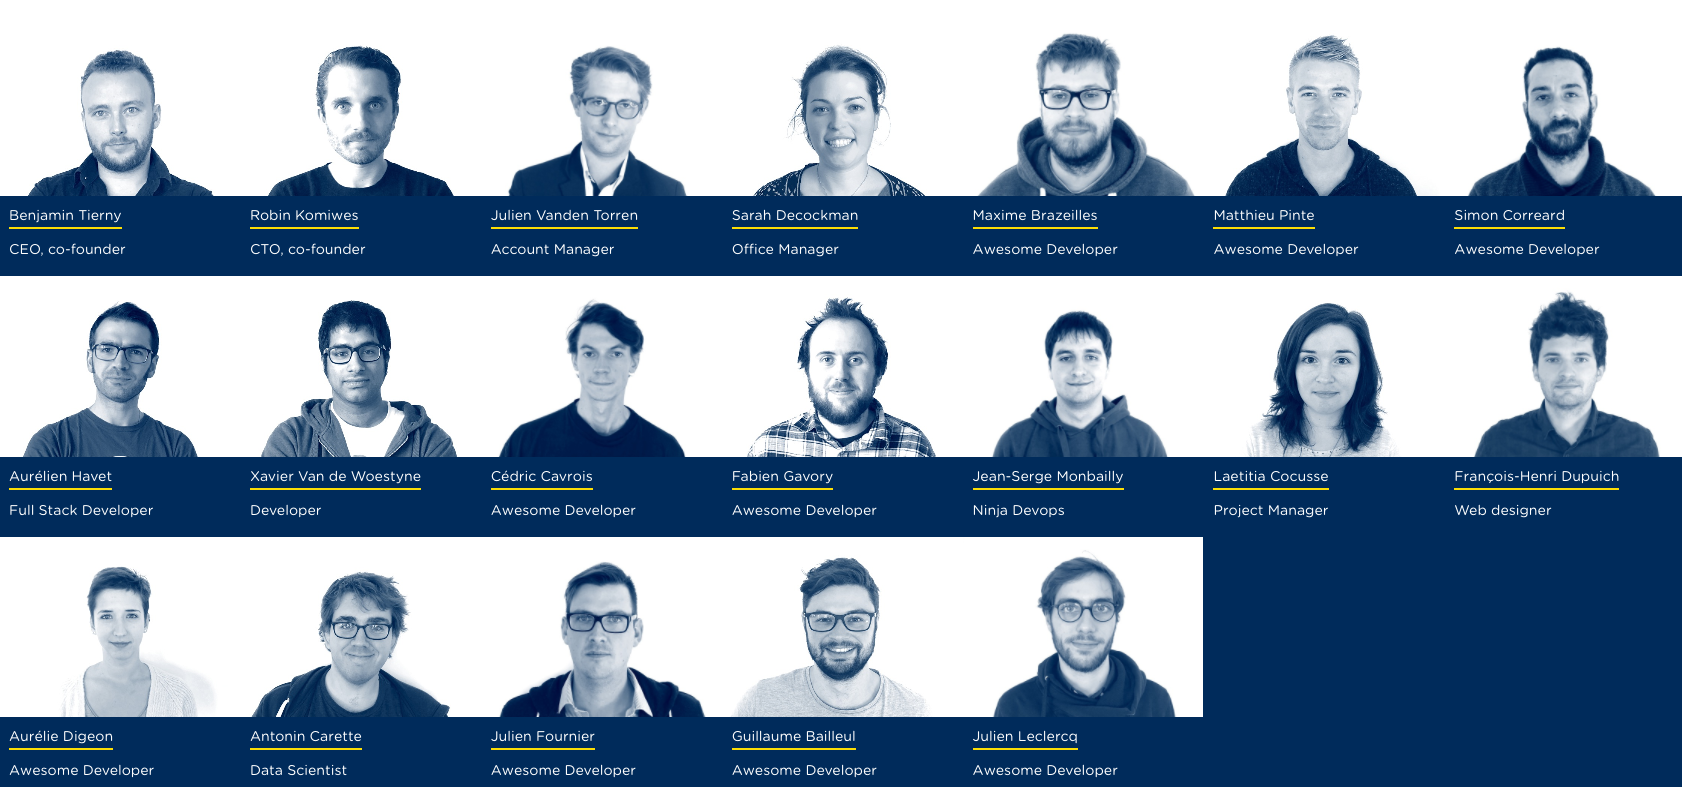
\includegraphics[height=6cm]{figures/team.png}
  \caption{L'équipe de Dernier Cri}
\end{figure}

\bigskip

\emph{Dernier Cri} est une entreprise à taille humaine. Cela se traduit
par des cycles de décision courts, des dirigeants plus accessibles et la
volonté de travailler dans un esprit d'équipe.

\bigskip

\emph{Dernier Cri} posséde une organisation souple qui offre
l'opportunité à tous ses employés de s'impliquer dans des projets
variés, que ce soit pour des clients ou bien en interne
(\emph{side-project}).

\bigskip

Au sommet de l'organisation de l'entreprise se trouve les deux
fondateurs, Benjamin Tierny (\emph{CEO}) et Robin Komiwes (\emph{CTO}),
ainsi que le troisième associé, Julien Vanden Torren (\emph{Account
manager}).

\bigskip

L'entreprise compte aujourd'hui 19 employés, dont trois associés, une
assistante de direction, une chef de projet et 14 développeurs. L'équipe
de développeurs est aussi constituée d'un \emph{devops}, et d'un
\emph{data scientist}. Grâce à de nombreux nouveaux projets, elle se
trouve dans une phase d'expension, avec de nouvelles embauches en
perspective.

\bigskip

Selon la demande, et les compétences recherchées par un client, il peut
arriver que des développeurs travaillent sur plus d'un projet à la fois,
des équipes de deux à trois développeurs sont donc créées, mélangeant
les compétences de chacun.

\bigskip

La gestion de projet peut se séparer en deux: la relation client, et la
gestion de projet en interne. Le chef de projet s'occupe de gérer la
première en récoltant les besoins du clients tout au long du projet, la
seconde se fait principalement par l'intermédiaire de \emph{Github}, que
le chef de projet tient à jour pour permettre aux développeurs d'être
efficaces. Ces deux points seront développés plus loin dans le rapport.

\bigskip

\emph{Dernier Cri} a à coeur de développer une culture entreprenariale
et informatique, c'est pourquoi s'est developpé des présentations
internes (dont certaines sont diffusées via une chaine youtube) ainsi
que des présentations publiques par l'intermédiaire d'articles de blog.

\subsubsection{Présentations internes}\label{pruxe9sentations-internes}

\begin{figure}[h]
  \centering
  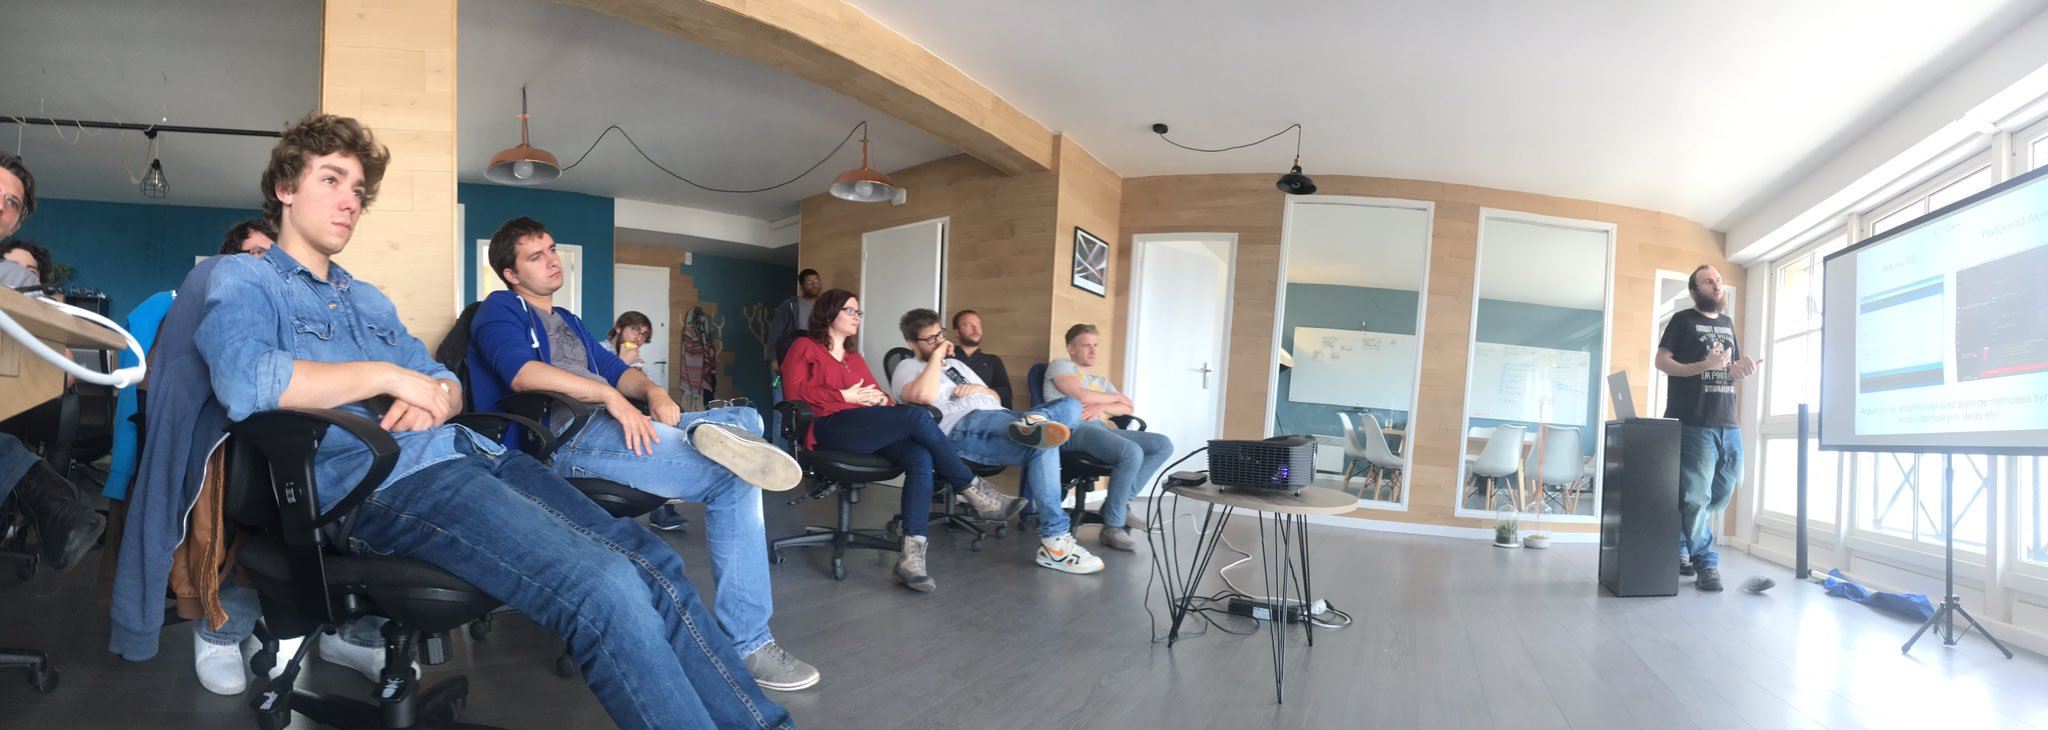
\includegraphics[height=4cm]{figures/talk.jpg}
  \caption{Fabien présentant comment fabriquer son propre hardware}
\end{figure}

\bigskip

Dans l'optique d'un partage du savoir dans l'entreprise, les employés
sont invités à faire des petites présentations (\emph{talks}) sur une
technologie, le resultat d'une veille, ou certains enjeux et solutions
techniques en rapport avec la réalisation d'un projet. Ces \emph{talks}
ont pour objectifs de partager aux collègues des expériences passées
et/ou des passions.

\bigskip

Ces présentations ont trois principaux avantages pour les spectateurs:

\begin{enumerate}
\def\labelenumi{\arabic{enumi}.}
\tightlist
\item
  permettre aux spectateurs de la présentation d'apprendre de nouvelles
  choses - c'est ainsi l'occasion de découvrir un sujet dont on ne se
  doutait pas de l'intéret ou de l'existence ;\\
\item
  sensibiliser ses coéquipiers à des problèmes, ou des technologies, qui
  peut être un véritable gain de temps dans le futur - la présentation
  est travaillée et structurée, c'est ainsi souvent beaucoup plus facile
  d'aborder un sujet avec ces \emph{talks}, que de devoir effectuer une
  recherche d'information sur divers supports ;\\
\item
  mutualiser la communication, et éviter de devoir expliquer
  individuellement les concepts.
\end{enumerate}

\bigskip

De même, l'orateur, par l'intermédiaire de sa présentation, doit devenir
un expert sur le sujet qu'il va couvrir. En effet, il devra assez
approfondir le sujet pour être capable, d'une part d'être clair dans sa
présentation, et d'autre part de répondre aux éventuelles questions
posées à la suite de cette dernière.\\
Ainsi, c'est pour lui une occasion de travailler sur ces compétences
d'orateur.

\bigskip

Un \emph{talk} interne peut faire office d'incubation pour une
présentation dans un autre contexte, afin de certifier l'intérêt du
sujet, de sonder les angles d'approfondissement possibles, de valider la
prestance de l'orateur.\\
En effet, il existe à Lille de nombreux évènements où il est possible de
faire des présentations (\emph{Meetups}, \emph{Take Off}, etc), ce qui
est très intéréssant mais aussi peut être assez intimidant. L'orateur
peut donc s'entraîner en interne, avant de l'ouvrir à la communauté.

\bigskip

Pendant mon stage j'ai eu l'occasion d'assister à des présentations sur
de nombreuses technologies telles que \emph{ReactJS}, \emph{Docker},
\emph{Rust}, \emph{MJML}, ou encore la fabrication d'un audit sur le
traitement de grosses données pour une \emph{startup} en pleine
expension.\\
La grande majorité de ces présentations sont publiées et ouvertes au
public sur la
\href{https://www.youtube.com/channel/UCDfdBlzldhg_PEu3xZTPsHg}{chaîne
youtube \emph{Dernier Cri}}.

\bigskip

\subsubsection{Article de blog}\label{article-de-blog}

\bigskip

Dernier Cri posséde également un
\href{http://derniercri.io/tech-blog}{blog technique}, alimenté par les
développeurs de l'équipe. Les objectifs sont sensiblement les mêmes que
pour les présentations internes. C'est sur ce point que \emph{Dernier
Cri} fait le plus de communication externe, afin de rayonner, démontrer
ses compétences techniques, et son esprit d'analyse.\\
Le blog technique permet ainsi à Dernier Cri de se positionner en tant
qu'expert.

\bigskip

Un blog est également utile pour tenir informée sa clientelle : il
permet de rester en contact permanent avec ses prospects, et de les
tenir au courant de l'actualité de l'entreprise, comme un nouveau
produit, la maitrise d'une nouvelle technologie, etc.

\bigskip

Pour le rédacteur de l'article, cela a également de nombreux avantages.
Par exemple, cela lui permet de travailler sa rédaction et son
argumentation, de partager avec d'autres développeurs à travers les
commentaires, de gagner en visibilité et en réputation, ou encore de se
forcer à rester à la page, afin de rester exhaustif et à jour dans ses
références.

\bigskip

J'ai eu l'occasion lors de mon stage d'écrire un article pour le blog
technique de \emph{Dernier Cri}. Dans cet article je décris les
technologies que j'ai utilisé lors de mon stage, \emph{ReactJS} et
\emph{Redux}, ainsi que cinq outils que j'ai découvert et qui ont
facilité le développement de mes projets.\\
Ce fut une expérience très enrichissante, car cela m'a poussé à enrichir
mes connaissances dans le domaine du web, de clarifier les concepts pour
savoir les expliquer à tous et de travailler ma qualité de rédaction.

\newpage

\section{Cadre du stage}\label{cadre-du-stage}

\bigskip

Pendant mon stage, j'ai participé au développement de deux applications
web : \emph{Photolix} et \emph{FinFrog}. Ces deux projets s'appuient sur
le framework \emph{ReactJS}, une bibliothèque \emph{JavaScript}
\emph{open-source} développée par Facebook depuis 2013. N'ayant jamais
utilisé cette bibliothèque, j'ai donc dû tout d'abord me former à
l'écosystème \emph{React}.

\bigskip

\subsection{Formation}\label{formation}

\bigskip

Je me suis formée sur \emph{Javascript ES6}, \emph{ReactJS} ainsi que
\emph{Redux}, car l'entreprise avait prévu de me confier des projets qui
utilisent ces technologies.\\
Cette formation s'est faite à partir du site
\href{https://www.codeschool.com/}{Code school}, qui dispose de cours
vidéos et d'exercices interactifs. De même, j'ai également pu compter
sur Fabien Gavory, un développeur de \emph{Dernier Cri} spécialisé dans
la technologie \emph{ReactJS}, pour m'aider et m'expliquer certains
concepts difficiles.

\bigskip

La popularité de ces trois technologies est en forte hausse, et elle
sont de plus en plus utilisées pour la création facile, rapide et
moderne d'applications web. C'est pourquoi ce fut une véritable chance
d'apprendre ces deux \emph{frameworks} lors de ce stage.

\bigskip

\subsubsection{Javascript ES6}\label{javascript-es6}

\bigskip

\emph{JavaScript} est un langage de programmation orienté web (pages web
dynamiques et serveur grâce à \emph{NodeJS}), devenu incontournable.
Créé en 1995 par Brendan Eich, il servait principalement à la
réalisation d'animations. Aujourd'hui, il est au centre des
applications, car avec ce langage que nous pouvons désormais contrôler
la totalité de ces dernières.\\
Cette montée en popularité s'est faite brusquement avec l'arrivée du
moteur \emph{V8} de Google, qui est au centre de Chromium. Ce langage
n'étant pas prévu à la base pour créer une application web, la syntaxe
de \emph{JavaScript} est complexe et lourde. C'est dans ce contexte
qu'une mise à jour du langage s'est imposée: \emph{ES6}.

\bigskip

\emph{ES6} (\emph{ECMAScript Edition 6}, ou encore \emph{ES2015}) a été
publiée en Juin 2015.\\
Elle ajoute un ensemble de normes à celles déjà présentes, afin
d'améliorer des fonctionnalités existantes dans \emph{ES5}, et d'en
apporter de nouvelles qui permettent d'alléger le code, ou de mieux le
structurer.\\
Ce tout permet de rendre le code source de l'application plus
maintenable, tout en restant compatible avec les précédentes versions de
\emph{JavaScript}.

\bigskip

Voici quelques nouveautés notoires de \emph{ES6} :

\begin{itemize}
\item
  L'introduction du mot-clef \emph{let} : tout comme le mot-clef
  \emph{var}, présent dans les anciennes versions de JavaScript, il
  permet de déclarer une variable, mais celle-ci reste limitée à la
  portée d'un bloc - c'est-à-dire que la variable ne peut être utilisée
  que dans le bloc où elle a été déclarée.
\item
  Les littéraux de gabarits (\emph{Template Literals}): ils
  correspondent à une technique d'intégration d'expressions, à
  l'intérieur de chaînes de caractères. Par rapport aux anciennes
  versions de JavaScript, ils sont une alternative aux concaténations,
  qui n'étaient pas pratiques et lisibles (voir exemple ci-dessous).

\begin{Shaded}
\begin{Highlighting}[]
\CommentTok{// ES6}
\KeywordTok{let} \NormalTok{name }\OperatorTok{=} \StringTok{"Aurélie"}
\KeywordTok{let} \NormalTok{result }\OperatorTok{=} \VerbatimStringTok{`Voici le rapport de }\SpecialCharTok{$\{}\NormalTok{me}\SpecialCharTok{\}}\VerbatimStringTok{.`}
\CommentTok{// ES5}
\KeywordTok{var} \NormalTok{me }\OperatorTok{=} \StringTok{"Aurélie"}\OperatorTok{;}
\KeywordTok{var} \NormalTok{result }\OperatorTok{=} \StringTok{"Voici le rapport de "} \OperatorTok{+} \NormalTok{me}\OperatorTok{;}
\end{Highlighting}
\end{Shaded}
\item
  Les paramètres par défaut: auparavant, pour définir une valeur par
  défaut pour un paramètre donné, il fallait tester si ce paramètre
  avait bien une valeur définie (différente de \texttt{undefined}), et
  lui affecter une valeur choisie le cas échéant. \emph{ES6} permet de
  faire cela directement lors de sa définition, avec une syntaxe plus
  concise.

\begin{Shaded}
\begin{Highlighting}[]
\CommentTok{// ES6}
\KeywordTok{function} \AttributeTok{f} \NormalTok{(x }\OperatorTok{=} \DecValTok{0}\OperatorTok{,} \NormalTok{y }\OperatorTok{=} \DecValTok{0}\NormalTok{) }\OperatorTok{\{}
    \ControlFlowTok{return} \NormalTok{x }\OperatorTok{+} \NormalTok{y}
\OperatorTok{\};}
\CommentTok{// ES5}
\KeywordTok{function} \AttributeTok{f} \NormalTok{(x}\OperatorTok{,} \NormalTok{y) }\OperatorTok{\{}
    \ControlFlowTok{if} \NormalTok{(x }\OperatorTok{===} \KeywordTok{undefined}\NormalTok{)}
        \NormalTok{x }\OperatorTok{=} \DecValTok{0}\OperatorTok{;}
    \ControlFlowTok{if} \NormalTok{(y }\OperatorTok{===} \KeywordTok{undefined}\NormalTok{)}
        \NormalTok{y }\OperatorTok{=} \DecValTok{0}\OperatorTok{;}
    \ControlFlowTok{return} \NormalTok{x }\OperatorTok{+} \NormalTok{y}\OperatorTok{;}
\OperatorTok{\};}
\end{Highlighting}
\end{Shaded}
\item
  Initialisateur d'objets: il arrive souvent de vouloir utiliser des
  variables comme propriétés d'un objet. \emph{ES6} introduit une
  notation permettant d'utiliser le nom de la variable comme nom de la
  propriété de l'objet créé.

\begin{Shaded}
\begin{Highlighting}[]
\CommentTok{// ES6}
\NormalTok{obj }\OperatorTok{=} \OperatorTok{\{} \NormalTok{x}\OperatorTok{,} \NormalTok{y }\OperatorTok{\}}
\CommentTok{// ES5}
\NormalTok{obj }\OperatorTok{=} \OperatorTok{\{} \DataTypeTok{x}\OperatorTok{:} \NormalTok{x}\OperatorTok{,} \DataTypeTok{y}\OperatorTok{:} \NormalTok{y }\OperatorTok{\};}
\end{Highlighting}
\end{Shaded}
\item
  Affectation par décomposition: pour accéder aux valeurs des propriétés
  d'un objet, il fallait pour cela itérer sur ces propriétés, ce qui
  était fastidieux et gourmand en lignes de code. \emph{ES6} a introduit
  une notation permettant de faire cela facilement, de façon compacte et
  implicite:

\begin{Shaded}
\begin{Highlighting}[]
\CommentTok{// ES6}
\KeywordTok{var} \OperatorTok{\{} \NormalTok{a}\OperatorTok{,} \NormalTok{b}\OperatorTok{,} \NormalTok{c }\OperatorTok{\}} \OperatorTok{=} \AttributeTok{someFunction}\NormalTok{()}
\CommentTok{// ES5}
\KeywordTok{var} \NormalTok{tmp }\OperatorTok{=} \AttributeTok{someFunction}\NormalTok{()}\OperatorTok{;}
\KeywordTok{var} \NormalTok{a  }\OperatorTok{=} \VariableTok{tmp}\NormalTok{.}\AttributeTok{a}\OperatorTok{;}
\KeywordTok{var} \NormalTok{b }\OperatorTok{=} \VariableTok{tmp}\NormalTok{.}\AttributeTok{b}\OperatorTok{;}
\KeywordTok{var} \NormalTok{c }\OperatorTok{=} \VariableTok{tmp}\NormalTok{.}\AttributeTok{c}\OperatorTok{;}
\end{Highlighting}
\end{Shaded}
\item
  Les \emph{arrow functions}: elles offrent une syntaxe plus courte,
  sont des fonctions anonymes (une fonction n'ayant pas de nom) et
  partage le contexte de leur parent.

\begin{Shaded}
\begin{Highlighting}[]
\CommentTok{/* fonction anonymes classique */}
\KeywordTok{let} \NormalTok{multiple }\OperatorTok{=} \KeywordTok{function} \NormalTok{(value) }\OperatorTok{\{}  
  \ControlFlowTok{return} \NormalTok{value }\OperatorTok{*} \DecValTok{10}
\OperatorTok{\}}
\CommentTok{/* arrow function */}
\KeywordTok{let} \NormalTok{multiple }\OperatorTok{=} \NormalTok{value }\OperatorTok{=>} \NormalTok{value }\OperatorTok{*} \DecValTok{10}  
\end{Highlighting}
\end{Shaded}
\end{itemize}

\bigskip

Étant donné que \emph{ES6} n'est pas encore totalement supporté par les
navigateurs, il est donc utile d'utiliser un transcompilateur vers
\emph{ES5}, comme le fait \emph{Babel.js}. Un transcompilateur permet de
prendre le code d'un langage de programmation comme son entrée, et de
récupérer en sortie le code dans un autre langage.\\
Ici, \emph{Babel.js} va traduire les particularité syntaxiques de
\emph{ES6} en \emph{ES5}.

\bigskip

L'apprentissage de \emph{ES6} a était primordial pour mon stage : les
nouvelles normes rendent vraiment le code plus facile à lire et à
écrire. J'ai ainsi, dès le début de mon stage, pu prendre de bonnes
habitudes quant au style de mon code.

\bigskip

En effet, j'ai eu l'occasion durant ce stage de travailler sur un projet
\emph{JavaScript} n'utilisant pas \emph{ES6} et j'ai eu de grandes
difficultés à me passer des facilités d'écritures. J'ai ainsi pu me
rendre compte que, sans \emph{ES6}, le code est beaucoup plus long et
laborieux à lire et à écrire.

\bigskip

Cela m'a également permis de me familiariser avec les normes
\emph{ECMAScript}, composant les différentes versions du langage
\emph{JavaScript}, et de me persuader de la nécessité de rester
attentive aux différentes actualités et évolutions des langages.\\
En effet, dans le milieu de l'informatique, les normes et les
\emph{frameworks} utilisés changent très souvent, et il est donc
important de rester attentif à l'actualité.

\bigskip

\subsubsection{React}\label{react}

\bigskip

Développée depuis 2013 par Facebook, \emph{React} est une bibliothèque
JavaScript déclarative, efficace et flexible pour la création
d'interfaces utilisateurs. Cette bibliothèque s'est démarquée notamment
par ses performances. Elle est aujourd'hui utilisée par de nombreuses
entreprises telles que \emph{Netflix}, \emph{Yahoo}, \emph{Airbnb} ou
encore \emph{Sony}.

\bigskip

Tout d'abord, React est basé sur l'utilisation d'un \emph{DOM}
(\emph{Document Object Model}) Virtuel. Le DOM est l'\emph{API} qui
permet au développeur web d'accéder et de manipuler le contenu d'une
page web. Cette \emph{API} founit une représentation structurée et
orientée objet de votre document. Elle fournit également des méthodes
pour l'ajout et la suppression d'éléments ainsi que la gestion des
événements, ce qui permet de créer du contenu dynamique. Le problème est
que la mise à jour du DOM, pour appliquer des modifications, est lente,
il est donc nécessaire de limiter les interactions avec celui-ci lors de
l'application de modifications. \bigskip

Grâce à l'utilisation d'un \emph{DOM} virtuel, un composant React ne
crée pas de \emph{HTML} mais une représentation sous forme d'objets et
de nœuds de ce à quoi le \emph{HTML} final doit ressembler. React va
comparer cette représentation au \emph{DOM} réel et en déduire les
opérations minimales à exécuter pour que les deux soient identiques.
Avoir une représentation sous forme d'arbre en JavaScript permet de
réaliser beaucoup plus d'opérations, d'utiliser les meilleurs
algorithmes de comparaison d'arbres et de faire toutes les modifications
du \emph{DOM} en une opération plutôt qu'au fur et à mesure.

\bigskip

Une autre particularité de \emph{React} est de découper l'application en
composants, dépendant d'un état. C'est après un changement de cet état
que \emph{React} déduit les changements à effectuer sur le \emph{DOM}.

\bigskip

Il faut noter que les composants sont des classes, héritant de
\texttt{React.Component}. Un composant \emph{React} possède deux types
de données :

\begin{itemize}
\tightlist
\item
  des paramètres (\emph{props}) immutables définis à leur instanciation,
  qui ne peuvent être manipulés qu'à l'extérieur du composant;
\item
  un état (\emph{state}), permettant le dialogue avec l'utilisateur. Cet
  état ne peut être modifié qu'à l'intérieur du composant;
\end{itemize}

\bigskip

Pour illustrer cette architecture, prenons l'exemple d'une simple
application \emph{Todo list}. Elle possède trois composants : la
\emph{todo liste} (\texttt{TodoListApp}), le formulaire d'ajout
(\texttt{TodoForm}) et l'affichage de la liste (\texttt{TodoItems}). Le
composant principal est la liste, qui possède la logique et les données
de l'application. Elle passe ses fonctions et ses données a ses
composants enfants, selon leur besoin.

\begin{verbatim}
class TodoListApp extends React.Component {
  constructor(props) {
    super(props);
    this.state = { items: [] };
  }

  addItem(element) {
    var itemArray = this.state.items;
    itemArray.push(element);
    this.setState({ items: itemArray });
    e.preventDefault();
  }

  render() {
      return (
        <div className="todoList">
          <TodoForm onSubmit={this.addItem} />
          <TodoItems items={this.state.items}/>
        </div>
      );
    }
}
\end{verbatim}

Le formulaire utilisera la fonction \texttt{addItem} de TodoListApp pour
modifier la liste. Cette modificaton de la liste déclenchera la
modification du composant TodoItems, puisqu'il reçoit la liste comme
\emph{props}.

\bigskip

Cette bibliothèque est aujourd'hui en expansion. Elle a un succès
certain auprès de la communauté des développeurs web, et de nombreux
outils se développent autour. C'est donc un avantage d'avoir pu
apprendre \emph{React} lors de mon stage, puis d'avoir mis en pratique
ces connaissances lors des deux projets que j'ai effectué.

\bigskip

\subsubsection{Redux}\label{redux}

\bigskip

En plus de \emph{React}, Facebook a fourni une architecture appelée
\emph{Flux} pour la gestion des donnés et la communication des
composants. Cette architecture promet un flot unilatéral des données
pour que le développeur puisse facilement suivre le trajet des données
d'un événement et ses conséquences.

\bigskip

Avec Flux, l'application va se décomposer de la façon suivante :

\begin{itemize}
\tightlist
\item
  des \emph{stores} qui sont l'endroit où les données sont concervées ;
\item
  des \emph{actions} qui représente l'ensemble des modifications
  possible ;
\item
  un \emph{dispatcher} qui notifie les stores des actions effectuées ;
\item
  des vues, les composants, qui vont transformer et afficher les données
  qu'on leur donne.
\end{itemize}

\bigskip

\emph{Redux} est une des implémentations de \emph{Flux} les plus
populaires, créée en Mai 2015 par Dan Abramov. Bien que reprenant les
concepts de \emph{Flux}, \emph{Redux} les simplifient en utilisant des
concepts liés à la programmation fonctionnelle.

\bigskip

La mise en place de \emph{Redux}, ou de \emph{Flux} en général peut
sembler dans un premier temps laborieuse, car elle impose de nombreux
fichiers, de nombreux composants différents et une façon de penser qui
peut désarçonner au début. Mais une fois les bases mises en place, cette
architecture a l'avantage d'offrir une bonne lisibilité quant aux
changements d'état. Il est possible de se retrouver dans le code très
rapidement et d'ajouter des composants sans difficultés puisque
\emph{React} et \emph{Flux} sont conçus pour être modulable. Flux trouve
donc son utilité dans les grandes applications.

\bigskip

Bien que \emph{Redux} soit la seule implémentation de \emph{Flux} que
j'ai eu l'occasion d'utiliser, après m'étre beaucoup documenté et avoir
discuté des différentes implémentations avec mes collègues (qui ont eu
l'occasion de l'utiliser sur des projets), je pense qu'il s'agit d'une
des meilleures. \emph{Redux} permet d'appréhender certain concept de la
programmation fonctionnel, est simple à utiliser et assez populaire pour
offrir un support de la communauté en cas de problème.

\bigskip

\begin{figure}[h]
  \centering
  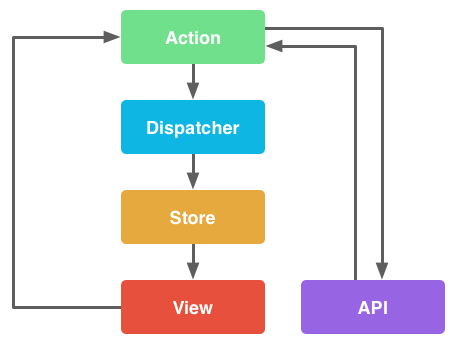
\includegraphics[height=5cm]{figures/react.png}
  \caption{Flux entre les différents composants}
\end{figure}

\subsection{Gestion de projet}\label{gestion-de-projet}

Le processus de développement d'une application pour un client possède
deux aspects fondamentaux. Tout d'abord il est nécessaire de mettre en
place une bonne relation client, d'un part pour bien comprendre les
besoins et les contraintes, d'autre part pour vérifier au fur et à
mesure du développement que la solution developpée correspond bien. Le
chef de projet reste en contact, plus ou moins régulierement, avec le
client pour présentation l'avancement et receuillir les retours.

\bigskip

Le deuxième aspect de la gestion de projet est l'organisation interne.
Une fois les besoins du client récoltés, il est nécessaire de mettre en
place une méthodologie pour répartir les tâches, suivre leur avancement
et vérifier la qualité du livrable.

\bigskip

\subsubsection{Relation client}\label{relation-client}

\bigskip

Lors du début du projet, le chef de projet discute avec le client pour
comprendre ses besoins et ses attentes. Aidé par le \emph{CEO}, il
essaye de conceptualiser une solution au problèmes du client, en
dégageant du discout du client des fonctionnalités techniques à mettre
en place. A partir de l'analyse de la demande, ils conceptualisent le
projet (diagramme de séquence, MCD, et architecture logicielle) et le
valident auprès du client avant de débuter les développements. Selon les
besoins, le chef de projet organise une réunion avec le(s)
developpeur(s) et le client pour clarifier certains points ou pour
discuter des différents approches du problèmes possible. C'est
l'occasion pour le développeur de comprendre la problèmatique métier qui
sera au coeur du projet, et de proposer des solutions, peut être un peu
différentes de celles imaginées par le client. En effet, le développeur
à souvent une approche différente du client: il peut proposer des
solutions légérements différentes mais beaucoup moins longues à mettre
en place techniquement, ou bien proposer des solutions techniques dont
le client ignoré l'existence.

\bigskip

Après cette première étape, le chef de projet peut diviser les
fonctionnalités en tâches et les faire estimer par un développeur. Il
estime le temps qu'il pense passer sur le problème, en prenant en compte
l'exploration de l'existant, le développement en lui-même, les tests et
les possibles retours. Cette estimation devra ensuite être validée par
le client. Elle sert notamment quand le projet est forfait. Dans ce type
de projet, si les développeurs dépassent l'estimation donnée, le surplus
n'est pas facturé, contrairement au projet en régie.

\bigskip

Il est ensuite temps de commencer le développement du projet. Il est
nécessaire de s'assurer tout au long du projet, que le produit en cours
de réalisation correspond aux attentes du client. C'est pourquoi un
environnement de \emph{staging} est mis en place. Un espace de
\emph{staging} est un environnement identique à celui de l'application
finale, mais utilisant de fausses données, où sont déployées les
nouvelles fonctionnalités. Il permet au client de tester et valider les
nouvelles fonctionnalités avant la mise en production.

\bigskip

Il est également courant de mettre en place des outils de
\emph{monitoring} pour assurer d'une part des performances, en termes de
temps de réponse par exemple, et d'autre part la qualité du code. Pour
cela \emph{Dernier Cri} utilise des outils tel que \emph{Papertrail}, ou
\emph{New Relic}.

\bigskip

\subsubsection{Organisation interne}\label{organisation-interne}

\bigskip

Une fois le projet découpé en fonctionnalités puis en tâches - où sont
listés l'ensemble des fonctionnalités à intégrer, et comportement
souhaité -, estimées et validées, une seconde phase de gestion de projet
commence. C'est la gestion interne du projet.

L'entreprise utilise principalement la plateforme \emph{Github}, pour
héberger le code de ses projets, et donc le logiciel de gestion de
versions \emph{Git}. \emph{Github} est une interface web permettant
d'interfacer avec des projets versionnés, et composés de multiples
applications aidant à la gestion de projets.

\bigskip

C'est sur un de ses outils que le chef de projet crée des \emph{issues},
c'est à dire un descriptif de chaque tâche. Une interface en forme de
tableau permet de séparer les tâches en plusieures colonnes, par exemple
: \emph{A faire}, \emph{En cours}, \emph{Terminé}. Il est aussi possible
d'attribuer les tâches à un contributeur, ou encore de leur attribuer
des labels tel que \emph{Urgent}, \emph{Bug} ou encore une estimation de
temps quand à la réalisation de la tâche.\\
Cela permet à chacun d'avoir une vue d'ensemble du projet (chef de
projet et développeurs) et de connaitre les priorités. Il est également
possible de commenter chaque \emph{issue} pour, par exemple, demander
des précisions, ou faire remonter une erreur.

\bigskip

Pour protéger le projet actuel, stable, des nouvelles modifications tant
que celles-ci ne sont pas testées, le développeur crée une
\emph{branche} dans Github, c'est à dire une copie du projet qui
évoluera indépendamment de la branche principale. C'est sur cette
branche que seront faites les modifications destinées à implémenter la
nouvelle fonctionnalité.

\bigskip

C'est ensuite le moment de passer au développement à proprement parler.
Le développeur utilise un environnement de developpement sur son propre
ordinateur pour simuler l'environnement de production. Cela peut se
traduire par la création d'une base de données, ou la connexion à une
\emph{API} spéciale. Il faut faire attention à ce que les données
utilisées lors de la phase de développement n'aient pas d'impact sur
celles de production.

\bigskip

Quand le développeur estime avoir terminer la tâche, il crée une
\emph{Pull request} sur Github, c'est à dire demande à fusionner sa
version du projet, modifiée pour résoudre la tâche, avec la version
principale, stable. Il demande ensuite à ses collégues ayant des
compétences dans le langage utilisé de relire et de commenter cette
\emph{Pull request}. C'est l'occasion pour les développeurs d'avoir
l'avis de leurs collégues sur leur style d'écriture et leur façon de
coder, ce qui permet souvent de découvrir de nouvelles méthodes et
d'argumenter sur les meilleurs techniques à utiliser. \emph{Dernier Cri}
utilise ce système de \emph{code review} pour garantir une certaine
qualité du code ainsi qu'un style d'écriture de code homogéne.

\bigskip

Une fois le développement de la fonctionnalité validé, la nouvelle
version du projet est déployé en \emph{staging}. Le chef de projet et,
si nécessaire, le client font une \emph{recette}, c'est à dire vérifie
que la version de \emph{staging} remplit bien le besoin exprimé par le
client, et que la nouvelle fonctionnalité n'a pas endommagé la version
existante. En cas de problème, le développeur revient sur la tâche
jusqu'à ce que tout soit réglé.

\bigskip

Une fois un lot de tâches effectuées, il est décidé en accord avec le
client de pousser les modifications sur la production. Il faut alors
vérifier que la \emph{mise en production} s'est bien passée : que le
site fonctionne toujours et que les nouvelles fonctionnalités sont bien
en place.

\newpage

\section{Mes réalisations}\label{mes-ruxe9alisations}

\bigskip

J'ai eu la chance de participer à plusieurs projets durant mon stage, de
façon plus ou moins importantes. Je vais commencer par vous présenter
les deux principaux projets sur lesquels je me suis investie.

\bigskip

Le premier projet auquel j'ai participé se nomme Photolix. C'est un site
internet de développement de photos, avec pour objectifs de toucher un
large public et de limiter au maximum le temps d'attente du client.

\bigskip

Le second projet est FinFrog, un site proposant des prêts financés par
des particuliers. Ce projet était déjà assez avancé à mon arrivé. Le
client possédait un site en ligne, mais souhaitait changer l'apparence
et ajouter des fonctionnalités, ce pourquoi il a fait appel à
\emph{Dernier Cri}.

\bigskip

Je vous présenterai également un outil que j'ai pu développer pour le
site de \emph{Dernier Cri}: un générateur d'image de partage des
articles sur les réseaux sociaux.

\bigskip

\subsection{Photolix}\label{photolix}

\subsubsection{Présentation et objectifs du
projet}\label{pruxe9sentation-et-objectifs-du-projet}

\bigskip

Dès mon arrivée dans l'entreprise j'ai été assigné à la réalisation
d'une application de développement photo. Le client possède un
laboratoire de développement photo sur Lille, et souhaitait proposer à
sa clientèle une application simple et efficace permettant de commander
le développement de photos.

\bigskip

Le principal objectif de ce projet était de télécharger les photos vers
le serveur au fur et à mesure de leur sélection, pour ainsi éviter le
temps d'attente du client lors de la saisie des informations dans le
tunnel de commande.

\bigskip

Lors de mon arrivée sur le projet, un développeur de \emph{Dernier Cri}
avait déjà posé des bases. Les fonctions de recadrage et de compression
de la photo était notamment déjà développées.

\bigskip

Les principaux objectifs du projet Photolix étaient les suivants :

\begin{itemize}
\tightlist
\item
  mettre en place le \emph{design} fournit par le client, à partir de
  maquette ;
\item
  gérer l'envoi des photos au serveur ;
\item
  mettre en place la possibilité de modifier les photos (formats,
  orientation\ldots{}) ;
\item
  pages de saisie des informations du client (adresses, informations de
  paiement) et page de remerciement.
\end{itemize}

\bigskip

\subsubsection{Outils utilisés}\label{outils-utilisuxe9s}

\bigskip

Lors de mon arrivée sur ce premier projet, j'ai du apprendre à utiliser
certains outils, tant au niveau de la gestion de projet, que du
développement en lui-même.

\bigskip

Tout d'abord, le projet utilise \emph{Github} pour héberger le code
source et pour la gestion de projet, et le logiciel de gestion de
versions \emph{Git}. Bien qu'ayant déjà utilisé \emph{Git} et
\emph{Github} lors de mon DUT informatique, de projets personnels ou
bien de projets à l'UTC, je ne connaissais pas certaines fonctionnalités
de Github utilisées par l'entreprise, notamment le code review et les
outils de gestion de projet.

\bigskip

Le projet déjà existant utilisait \emph{npm}, le gestionnaire de paquets
officiel de \emph{Node.js}. Il permet d'installer des applications
\emph{Node.js} disponibles sur le dépôt npm et gère les dépendances pour
une application. Il offre également la possibilité de créer des scripts.
C'est une option vraiment pratique car elle permet de construire et
lancer l'application en une commande.

\bigskip

Pour mon environnement de travail, j'ai aussi utilisé un \emph{linter}.
Le \emph{code linting} est un type d'analyse statique qui est
fréquemment utilisé pour trouver des modèles problématiques ou le code
qui ne respecte pas certaines directives de style. Concraitement, il
permet d'afficher dans un éditeur de texte les erreurs. Il existe des
\emph{linters} de code pour la plupart des langages de programmation, et
les compilateurs incorporent parfois le linting dans le processus de
compilation. J'ai personnellement utilisé \emph{ESLint}, qui est un
\emph{linter} JavaScript open-source, libre et qui permet aux
développeurs de créer leurs propres règles de filtrage.

\bigskip

J'ai également pu utiliser le \emph{chatops} de \emph{Dernier Cri}, un
outil d'administration système via la conversation. Intégré au
\emph{Slack} (une application de messagerie) de l'entreprise, il permet
à tout le personnel d'obtenir des informations sur un serveur ou une
application et d'effectuer des résolutions simples en cas de panne.
Concrêtement, j'ai principalement utilisé le chatops pour déployer mon
application.

\bigskip

L'application était écrite en \emph{React} avec l'utilisation de
\emph{Redux}. J'ai pu donc mettre en application les principes appris
lors de ma première semaine à \emph{Dernier Cri}.

\bigskip

Pour l'intégration du style du site, j'ai pu utiliser \emph{Zeplin}.
C'est une application de collaboration pour les designers et les
intégrateurs. Il permet aux designers de télécharger leurs maquettes
fonctionnelles directement à partir de \emph{Sketch}, un logiciel de
création de maquette, et les ajouter aux dossiers de projet dans
\emph{Zeplin}. Les annotations seront automatiquement ajoutées aux
designs (tailles, couleurs, marges et même suggestions CSS pour certains
éléments). Il est alors beaucoup plus simple pour le développeur
d'intégrer les maquettes.

\bigskip

Finalement, pour l'intégration des maquettes, j'ai fait le choix
d'utiliser \emph{SASS} (\emph{Syntactically Awesome Stylesheets}). C'est
un langage de génération dynamique de feuilles de style. On peut le voir
comme une extension de \emph{CSS3}, ajoutant de nouvelles règles dans
notre façon d'intégrer un design. Les principaux ajouts sont : les
variables, les \emph{mixins,} l'héritage de sélection et différents
options très utiles.

\bigskip

\subsubsection{Déroulement}\label{duxe9roulement}

\bigskip

\paragraph{Historique du projet}\label{historique-du-projet}

\bigskip

Le projet a été initialement développé par un autre développeur de
\emph{Dernier Cri}. Après avoir receuilli les besoins du client, il
avait fournit un premier jet, présentant le découpage du site, en
monopage.\\
Après ce premier rendu, le client a fait appel à un graphiste pour nous
fournir une maquette de l'application voulue. Après ce travail de
formalisation, il a été décidé que l'application contiendrait finalement
plusieurs pages.

\bigskip

\paragraph{Intégration des
maquettes}\label{intuxe9gration-des-maquettes}

\bigskip

La première partie du projet a consisté à intégrer les maquettes fournit
par le client. Dans un premier temps, j'ai du redécouper l'application.
En effet, lors du premier jet réalisé par mon collègue, le client était
parti sur une application monopage. Il a donc tout d'abord fallut mettre
en place un routeur pour permettre à l'utilisateur de naviguer entre les
pages.

\bigskip

J'ai choisi, après quelques recherches, d'utiliser React Router.
\href{https://github.com/ReactTraining/react-router}{React Router} est
une bibliothèque de routage pour React. Il dispose d'une \emph{API}
simple avec des fonctionnalités puissantes. Il garde l'interface
utilisateur synchronisé avec l'\emph{URL}. React Router est très simple
à utiliser. Il suffit de lister les différentes routes souhaitées,
associées au composant correspondant.

\begin{verbatim}
// Exemple de création de routes avec React-Router
import { Router, Route, hashHistory } from 'react-router'

render((
  <Router history={hashHistory}>
    <Route path="/" component={App}/>
    <Route path="/about" component={About}/>
  </Router>
), document.getElementById('app'))
\end{verbatim}

\bigskip

Une fois ce découpage effectué, j'ai mis en place SASS pour la gestion
des feuilles de style. Pour faciliter son utilisation, j'ai créé
plusieurs fichiers avec les variables et fonctions (mixins) qui seront
utilisés dans tout le projet. Le fichier contient notamment les codes
hexadecimaux des couleurs de l'application, les tailles des polices
d'écriture utilisées, etc. Utiliser des variables évite de devoir
revenir sur tous les fichiers du projet si l'on décide de changer l'une
de ses variables.

\bigskip

Une fois ces fichiers \emph{SASS} principaux créés, j'ai simplement créé
un fichier SASS pour chaque composant React de l'application, qui
contient donc tout le style de ce composant. J'ai du faire beaucoup de
recherches pour être à l'aise avec le \emph{CSS} (\emph{Cascading Style
Sheets}), c'est à dire le langage décrivant la présentation de
l'application.

\bigskip

L'intégration du style fut assez rapide, l'application étant
visuellement assez simple. Grâce à cette première étape j'ai pu me
familiariser avec l'organisation du projet avant d'attaquer des parties
plus difficiles.

\bigskip

\paragraph{Formatage et téléchargement des
photos}\label{formatage-et-tuxe9luxe9chargement-des-photos}

\bigskip

La deuxième partie du projet était centrée sur le téléchargement des
photos vers le serveur. Le client nous a fourni une \emph{API} assez
simple que nous devions manipuler pour envoyer les photos, changer le
nombre d'exemplaires, récupérer le prix de la commande\ldots{}

\bigskip

La majeur difficulté durant cette étape fut de ne pas avoir accès
directement à l'\emph{API}, le client préférant developper cette partie
de l'application lui-même. La conception de l'\emph{API}avait été
réalisé sans concertation avec les équipes \emph{front}, ce qui ne
permettait donc pas de supposer son fonctionnement et surtout comment
s'interfacer avec. De plus, la documentation fournie n'était pas
exhaustive et peu détaillée, il était souvent nécessaire de demander des
précisions ou des évolutions au client. Même si la communication était
assez rapide, le fait de ne pas avoir la main sur l'\emph{API} a ralenti
considérablement le développement.

\bigskip

Une autre difficulté était le redimensionnement des images avant l'envoi
au serveur. En effet, quand l'utilisateur sélectionne des photos, nous
devons tout d'abord passer la photo au format sélectionné, et donc gérer
les formats incompatibles. Cela a apporté beaucoup de questions. Par
exemple, si une photo est en 10x15 et que l'utilisateur a sélectionné le
format 11x15 que fait-on ? Coupe-t-on des morceaux de la photo pour
arriver au format voulu ? Ou bien conserve-t-on l'intégrité de la photo
en ajoutant des bandes ?

\bigskip

Cela a donc donner lieu à beaucoup de discussions avec le client pour
résoudre toutes ses problèmatiques avant de developper les solutions. La
fonction de redimensionnement est une fonction clé du projet. Une fois
la photo redimensionnée, nous réduisons la résolution de la photo
jusqu'a 300dpi (point par pouce). C'est la résolution optimale pour
l'impression de photo : assez élevée pour garantir une bonne qualité à
l'impression, et assez faible pour rendre le téléchargement vers le
serveur le plus rapide possible.

\bigskip

\paragraph{Modification des photos}\label{modification-des-photos}

\bigskip

L'étape suivante est la création de l'interface et des fonctions
permettant à l'utilisateur de modifier ses photos. Il peut changer le
format, recadrer la photo, changer l'orientation\ldots{} J'ai tout
d'abord chercher s'il existait déja un outil pour le recadrage de la
photo.

\bigskip

C'est à ce moment que j'ai découvert la diversité des outils React
proposés par la communauté : il est très facile de trouver des
composants sur Github qui correspondent à votre besoin. J'ai donc pu
utiliser
\href{https://github.com/roadmanfong/react-cropper}{\emph{react-cropper}},
trouvé sur \emph{Github} après quelques recherches, qui s'est révélé
très efficace. Il permet de gérer le recadrage, fournit des fonctions
renvoyant toutes les données intéressantes (dimensions du recadrage,
rotation de la zone de recadrage\ldots{}). Ce fut ma première
intégration d'un outil React.

\bigskip

Pour mettre en place mes autres fonctions de modification des photos,
j'ai surtout dû modifier la fonction principale de redimensionnement des
photos, utilisée lors du téléchargement initial. J'ai pu mettre en place
les modifications possible sur une photo demandées :

\begin{itemize}
\tightlist
\item
  Choix du format (10x15, 11x15 et 08x10);
\item
  Choix de l'orientation (portrait ou paysage) ;
\item
  Possibilité de recadrer la photo ;
\item
  Choix de concerver ou non l'intégrité de la photo ;
\end{itemize}

\bigskip

Enfin, il a fallut mettre en place l'interface utilisateur. Durant cette
étape nous avons beaucoup échangé avec le client pour essayer de trouver
la présentation la plus intuitive et pratique pour les utilisateurs de
\emph{Photolix}.

Un premier livrable a été fourni au client (toujours sur l'environnement
de staging) afin qu'il puisse effectuer des tests utilisateurs. Ces
tests on permit de remonter plusieurs informations : peu de
disfonctionnement nous ont été remonté ce qui est un point très
favorable , la grande majorité des retours sont des erreurs de
conception, rendant l'application peu confortable à l'usge. J'ai donc pu
reprendre le développement pour résoudre ces problèmes et rendre
l'application plus ergonomique et fonctionnel.

\paragraph{Pages informations des clients, paiement et
remerciement}\label{pages-informations-des-clients-paiement-et-remerciement}

\bigskip

La dernière partie du projet consistait à mettre en place les autres
pages de l'application, servant à récolter les informations nécessaires
à la commande, et à les envoyer à l'\emph{API}. Ces pages sont :

\begin{itemize}
\tightlist
\item
  La page de saisie des adresses, de livraison et de facturation ;
\item
  La page de paiements, soit par carte bancaire, soit par Paypal ;
\item
  La page de remerciements avec un récapitulatif de la commande, ainsi
  que des liens pour partager l'événement sur les réseaux sociaux.
\end{itemize}

\bigskip

Pour la page de saisie de l'adresse, ce fut l'occasion pour moi de créer
pour la première fois un formulaire en React et Redux. Avec ce
framework, la création de formulaire est assez peut instinctif car il
faut répercuter chaque changement des champs, chaque lettre écrite ou
effacée, pour que l'état de l'application soit toujours à jour. C'est
assez fastidieux et inhabituel.

\bigskip

Après cette première expérience dans la création de formulaire, j'ai pu
découvrir un outil, \emph{redux-form}, permettant de créer beaucoup plus
facilement des formulaires et gérant automatiquement la mise-à-jour de
l'état de l'application. J'ai pu utiliser cet outil dans mon second
projet. Mais je pense que le fait d'avoir d'abord dû faire toute
l'implémentation nécessaire par moi-même m'a permis de prendre
conscience des problèmatiques de cette pile technologique : le maintien
de l'état de l'application, la communication entre les composants etc.

\bigskip

J'ai ensuite travaillé sur le page de remerciement. Sur cette page, on
affiche un récapitulatif de la commande ainsi que des liens pour
partager l'évènement sur les réseaux sociaux. J'ai ainsi pu apprendre
comment partager sur Facebook et Tweeter un message, associé à une
\emph{URL}.

\bigskip

Finalement, sur les trois pages précédemment citées, j'ai dû faire
apparaître un récapitulatif de la commande, avec notamment le nombre de
photos commandées, le prix par photo, le prix total, ainsi que la
possibilité d'entrer un code de promotion avant le paiement. Cette
partie à demandée de la réflexion car le calculs des prix était
différent avant et après le paiement. En effet, dans l'absolu, il faut
récupérer le prix à partir de l'\emph{API}, pour être certain de son
exactitude. Cependant, avant le paiement il est possible que toutes les
photos ne soient pas encore envoyées à l'\emph{API}et donc le prix
renvoyé par celle-ci n'est pas définitif. Il est alors nécéssaire de
faire le calcul du prix dans l'application, et d'afficher ce resultat
dans le récapitulatif. Une fois le paiement effectué, il faut afficher
le prix envoyé par l'\emph{API}, puisqu'il s'agit du prix final.

\bigskip

\paragraph{Fin du projet}\label{fin-du-projet}

\bigskip

Vers mi-octobre, j'ai été réaffectée à un autre projet, laissant la fin
du projet \emph{Photolix} au collègue ayant commencé le projet. Celui-ci
a fini de mettre en place la gestion du téléchargement des photos vers
le serveur, notamment après leurs modifications. Il a également revu la
fonction de redimensionnement des photos, car celle utilisée au debut
n'était pas assez performante : ~si nous montions à une centaine de
photos chargées, le navigateur ne supportait pas la charge.

\bigskip

J'ai pu étudier les modifications apportées par mon collègue, et
apprendre des erreurs que j'ai pu commettre. Par exemple, je n'avais pas
assez travailler la gestion des erreurs. Il a fallut que mon collègue
reprenne mon travail pour ajouter l'affichage des erreurs, en cas par
exemple d'erreur lors du téléchargement des photos. Ces enseignements
m'ont permis de ne pas reproduire ces erreurs dans le second projet sur
lequel j'ai été affecté.\\
Cependant la majorité de mon développement était fonctionnel et n'a pas
nécéssité de retours de sa part.

\bigskip

Finalement, j'ai pu retravailler sur le projet en décembre. Après un
premier rendu au client, celui-ci souhaitait quelques corrections ainsi
que l'ajout de quelques fonctionnalités. Il avait utilisé un échantillon
d'utilisateurs pour tester l'application et avait relevé des
améliorations possibles à l'interface. J'ai donc pu aider Fabien à
mettre en place ces modifications.

\bigskip

Aujourd'hui \emph{Photolix} est en ligne et fonctionnel. L'équipe de
dévelopemment de \emph{Dernier Cri} reste à disposition en cas de
disfonctionnement ou d'améliorations souhaitées.

\subsubsection{Conclusion}\label{conclusion}

\bigskip

Ce premier projet chez \emph{Dernier Cri} m'a beaucoup apporté. Pour
commencer, j'ai pu me familiariser aves les méthodes de gestion de
projet de l'entreprise, le processus allant de la formalisation du
probléme, jusque sa mise en ligne. Dans le même temps j'ai pu prendre en
main les outils utilisés chez \emph{Dernier Cri}, tel que \emph{Github},
avec toute la gestion des différentes branches, les \emph{Pull Request}
ainsi que la gestion des issues etc. Ce fut une étape essentielle pour
mon intégration dans l'équipe de développement.

\bigskip

Ce projet m'a également permit d'apprendre à utiliser React et Redux.
Ces technologies sont aujourd'hui en pleine expansions, évolue beaucoup
et ont un bel avenir devant elles. J'ai également pu apprendre le
développement \emph{front-end}, alors que jusque là mes compétences
techniques étaient plus tournées vers du \emph{back}.

\bigskip

Evidemment, j'ai connu de nombreuses difficultés lors du développemment
de \emph{Photolix}. Mon inexpérience m'a conduite à faire des erreurs, à
fournir un résultat qui n'était pas optimal. J'ai heureusement pu
compter sur mon collégue présent sur le projet, pour me soutenir, me
corriger et rattraper certaines erreurs, surtout vers la fin du projet,
à travers le processus de \emph{code review} décrit précédemment. Grâce
à cela, j'ai pu mettre en place de meilleures pratiques durant le projet
suivant.

\bigskip

Finalement, c'est une vraie chance d'avoir pu travailler dès mon arrivée
sur un projet pour un client. J'ai ainsi été tout de suite confrontée
aux vraies problématiques du développement d'une application web, de la
relation cliente, avec des dates butoires et des évolutions des
spécifications en cours de projet.

\subsection{FinFrog}\label{finfrog}

\subsubsection{Présentation et objectifs du
projet}\label{pruxe9sentation-et-objectifs-du-projet-1}

\bigskip

Avec l'arrivée d'un nouveau client et la nécessité de fournir un
développeur \emph{React} sur son projet, j'ai quitté le projet
\emph{Photolix} pour rejoindre \emph{Finfrog}. L'équipe travaillant sur
ce projet était constituée d'une chef de projet, d'un \emph{devops}
chargé notamment de l'infrastruture et des déploiements de
l'application, et de moi-même pour le développement.

\bigskip

\emph{Finfrog} est un projet de prêt collaboratif, c'est à dire que le
site propose des prêts financés par des particuliers. L'objectif de
\emph{FinFrog} est de proposer des petits prêts, avec un remboursement
sur de petites mensualités, à des particuliers. Les prêts proposés vont
de 200 à 600 euros, à rembourser sur une durée d'un à trois mois.

\bigskip
La demande client était de réaliser une refonte du site. \emph{Dernier
Cri} a décidé d'accepter cet existant, de s'adapter à lui, et de pouvoir
le modifier, y ajouter les fonctionnalités souhaitées, sans devoir
repartir de zéro.

\bigskip

Le site était déjà en ligne, développé par un développeur de chez
\emph{FinFrog}. Il a été fermé le temps de réaliser les changements à la
demande du client.

\bigskip

La première demande était de mettre en place un nouveau design sur le
site, d'abord sur la page d'accueil, puis sur les formulaires de demande
de prêts (le chemin emprunteur).

\bigskip

Par la suite, j'ai été amené à developper de nouvelles fonctionnalités
pour \emph{Finfrog}, comme la partie du site réservée à la gestion des
prêts par l'administrateur, les espaces emprunteur et prêteur, la
génération de contrats.

\bigskip

\subsubsection{Outils utilisés}\label{outils-utilisuxe9s-1}

\bigskip

La projet \emph{Finfrog} utilisait principalement les même outils que
\emph{Photolix} : utilisation de \emph{npm} pour la gestion des paquets,
de \emph{Zeplin} pour étudier le design, de \emph{React} et
\emph{Redux}, etc.

\bigskip

Cependant à mon arrivée sur \emph{FinFrog}, le projet était hébergé sur
\emph{Bitbucket} et non pas \emph{Github}. Il a donc fallut que je
m'habitue à ce nouveaux gestionnaire, à son interface et ses
fonctionnalités différentes de \emph{Github}. Par la suite nous avons
migré le projet sur \emph{Github} afin d'accéder aux fonctionnalités de
gestion de projet qu'il fournit.

\bigskip

Sur ce projet, nous avions aussi en charge la partie \emph{API}et base
de données. L'\emph{API} est écrite en \emph{Nodejs} et la base de
donnée est une \emph{PostgreSQL}, donc manipulable en \emph{SQL}.
Cependant j'ai eu peu d'occasion de manipuler la base de donnée.

\bigskip

Finalement, pour lancer les processus du site et de l'\emph{API}, nous
avons utilisé \emph{PM2}. \emph{PM2} est un gestionnaire de processus de
production pour les applications \emph{Node.js}, avec un équilibreur de
charge intégré. Il vous permet de garder les applications en vie pour
toujours, de les recharger sans temps d'arrêt et de faciliter les tâches
administratives courantes du système.

\bigskip

\subsubsection{Déroulement}\label{duxe9roulement-1}

\paragraph{Page d'accueil et demande de
prêt}\label{page-daccueil-et-demande-de-pruxeat}

\bigskip

A mon arrivée sur le projet, \emph{Dernier Cri} était chargé de
l'intégration d'un nouveau \emph{design} pour le site déjà existant.
Cette intégration comprenait tout d'abord la page d'accueil, puis le
tunnel de demande de prêt.\\
Ce fut également l'occasion de m'adapter a l'organisation - tant au
niveau du code, que du processus de développement - du projet. Au début
de celui-ci, je n'avais accès qu'au code du côté \emph{front} de
l'application, tandis que le développeur du client gardait la main sur
l'\emph{API} ainsi que la partie du projet calculant les intérêts des
prêts.

\bigskip

L'intégration du nouveau \emph{design} de la page d'accueil fut une
bonne entrée en matière : elle était assez simple, principalement du
changement de couleur et d'images, pour mettre en place la nouvelle
identité visuelle de l'application. J'ai ainsi pu me familiariser avec
l'organisation du code source du projet ainsi que la logique métier
sous-jacente.

\bigskip

Après la page d'accueil, j'ai du m'occuper du tunnel de réservation. Sur
l'application existante, les fomulaires étaient déjà en place. Il était
question d'ajouter certain champs et de redécouper les formulaires selon
les nouvelles maquettes. Pour cela, j'ai du me plonger dans la partie du
site plus technique : la communication entre les composants, les pages,
les outils utilisés pour la gestion des formulaires, les appels à
l'\emph{API} pour récupéré les informations de l'utilisateur, et
enregistrer les modifications etc.

\bigskip

Pour la gestion des formulaires, le projet utilisait \emph{Redux Form},
un outil permettant de maintenir l'état du formulaire à jour dans le
\emph{store Redux}. Il suffit d'utiliser les composants et fonctions
fourni‡s par \emph{Redux Form} pour construire le formulaire. Cela se
concrétise principalement par deux éléments :

\begin{itemize}
\tightlist
\item
  une fonction
  \texttt{reduxForm(\{form:\ \textquotesingle{}formName\textquotesingle{}\})(TestForm)}
  où \emph{Testform} est un composant contenant le formulaire, et
  \texttt{formName} un nom unique, qui identifiera le formulaire dans le
  \emph{store}.
\item
  un composant \texttt{Field} qui connectera chaque champ du formulaire
  avec le \emph{store Redux}. Ce composant prend comme propriété un
  autre composant. Cela peut être un composant de base, comme
  \texttt{input} ou \texttt{select}, ou bien un composant personnalisé.
\end{itemize}

Avec ces deux éléments, il est simple de créer un formulaire :

\begin{verbatim}
import React from 'react'
import { Field, reduxForm } from 'redux-form'

const TestForm = (props) => {
  const { handleSubmit, pristine, submitting } = props
  return (
    <form onSubmit={handleSubmit}>
      <div>
        <label>First Name</label>
        <div>
          <Field
            name="email"
            component="input"
            type="text"
            placeholder="Email"/>
        </div>
      </div>
      <div>
        <label>Last Name</label>
        <div>
          <Field
            name="password"
            component="input"
            type="password"
            placeholder="Password"/>
        </div>
      </div>
      <div>
        <button type="submit" disabled={submitting}>
          Submit
        </button>
      </div>
    </form>
  )
}

export default reduxForm({
  form: 'testForm'
})(TestForm)
\end{verbatim}

\bigskip

Le tunnel des demandes de prêt est constitué de formulaires:

\begin{itemize}
\tightlist
\item
  Le descriptif du projet : l'utilisateur doit sélectionner la catégorie
  de son projet (travaux, voyages, meubles, etc.) ainsi que le type
  (personnel, professionel ou étude). Cette information est importante,
  non seulement pour pouvoir comprendre la catégorie d'utilisateur du
  site, mais surtout pour respecter les contraintes légales d'un prêt.
  En effet, le taux d'emprunt autorisé varie selon le type du prêt.
\item
  L'identité et les coordonnées de l'utilisateur : il doit fournir son
  identité (nom, prénom, date de naissance, etc.) ainsi que ses
  coordonnées. C'est également une contrainte légale.
\item
  Les dépenses et revenus : nous récupérons des informations sur les
  capacités financières de l'utilisateur pour évaluer sa capacité à
  rembourser le prêt.
\item
  Les coordonnées bancaires : l'utilisateur fournit les informations de
  sa carte bancaire ainsi que son IBAN, pour permettre le transfert de
  l'argent prêté dans un premier temps, puis le prélèvement des
  remboursements.
\item
  Le téléchargement de la pièce d'identité (carte d'identité, passeport,
  permis de conduire, etc.) : c'est également une obligation légale de
  vérifier l'identité de l'utilisateur.
\end{itemize}

\bigskip

C'est au terme de cette suite de formulaires que la demande de prêt est
créée. C'est donc une étape primordiale, puisqu'il faut s'assurer que
les utilisateurs n'abandonnent pas la demande en cours de route. Pour
observer le taux de rétention d'utilisateurs sur cette partie du site,
j'ai mis en place deux outils sur l'application :

\begin{itemize}
\tightlist
\item
  Tout d'abord le classique \emph{Google Analytics}, qui permet
  d'observer l'audience du site, heure par heure, page par page. On peut
  voir les caractéristiques des utilisateurs : leur système
  d'exploitation, navigateur, sexe, tranche d'âge, etc. ;
\item
  J'ai également mis en place \emph{hotjar}, un outil qui permet entre
  autre d'enregistrer les interactions entre l'internaute et une page
  web (clic, \emph{scroll}, mouvements de la souris, etc.). Cet outil a
  permis d'identifier un bon nombre de disfonctionnements de
  l'application, en observant les pages où l'utilisateur se retrouvait
  bloquer, ou passait trop de temps (par rapport au scénario
  initialement prévu).
\end{itemize}

\bigskip

Durant la modification de ce formulaire j'ai également dû mettre en
place le téléchargement de la pièce d'identité sur \emph{Amazon Simple
Storage Service} (\emph{Amazon S3}), qui est une solution de stockage
sur Internet. En effet, une fois la pièce d'identité envoyée à
l'\emph{API} de \emph{FinFrog}, nous la chargeons dans un stockage
externe, car la loi impose de pouvoir justifier de l'identité des
emprunteurs.

\bigskip

L'un des objectifs de cette première partie était de développer un site
\emph{responsive}, c'est à dire un site web dont la conception et le
développement vise à offrir le même confort visuel pour des supports
différents (comme les ordinateurs, smartphones, tablettes, etc.). Pour
arriver à cela, le client nous a fourni, pour chaque page du site, deux
maquettes différentes : une pour la version ordinateur et tablette, une
autre pour la version \emph{smartphone}.

\bigskip

Un autre point primordial du développement \emph{front} est la
compatibilité entre les navigateurs. En effet chaque navigateur dispose
de son propre « moteur d'affichage », et un même site pourra avoir un
affichage et un comportement très différent selon le navigateur utilisé.
La compatibilité multi-navigateurs consiste à essayer d'avoir un rendu
et un comportement identique d'un navigateur à l'autre.

\bigskip

Une première étape pour y arriver est de connaitre les navigateurs les
plus utilisés. Aujourd'hui, \emph{Chrome} est le navigateur le plus
utilisé (51\%), suivi par \emph{Safari} (18\%), \emph{Internet Explorer}
et \emph{Edge} (le nouveau navigateur de \emph{Microsoft}) (11\%).

\begin{figure}[h]
  \centering
  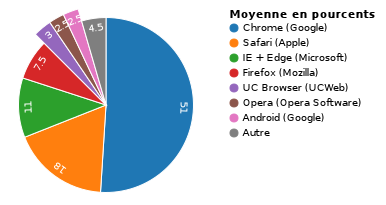
\includegraphics[height=4cm]{figures/browsers.png}
  \caption{Les parts de marché des navigateurs Web dans le monde, toutes plates-formes confondues (janvier 2017, source Wikipedia)}
\end{figure}

\bigskip

Une fois le site en ligne et visité par un nombre d'utilisateurs
suffisant, il est possible de connaître les navigateurs utilisés par ces
visiteurs, grâce à des outils comme \emph{Google Analytics}, qui
permettent d'analyser l'audience d'un site web. Pour \emph{FinFrog},
nous avons pu observer que \emph{Chrome} était bien le navigateur le
plus utilisé (63.71\%), suivi par \emph{Firefox} (14.81\%),
\emph{Internet Explorer} (8,54\%) et \emph{Safari} (8.22\%).

\begin{figure}[h]
  \centering
  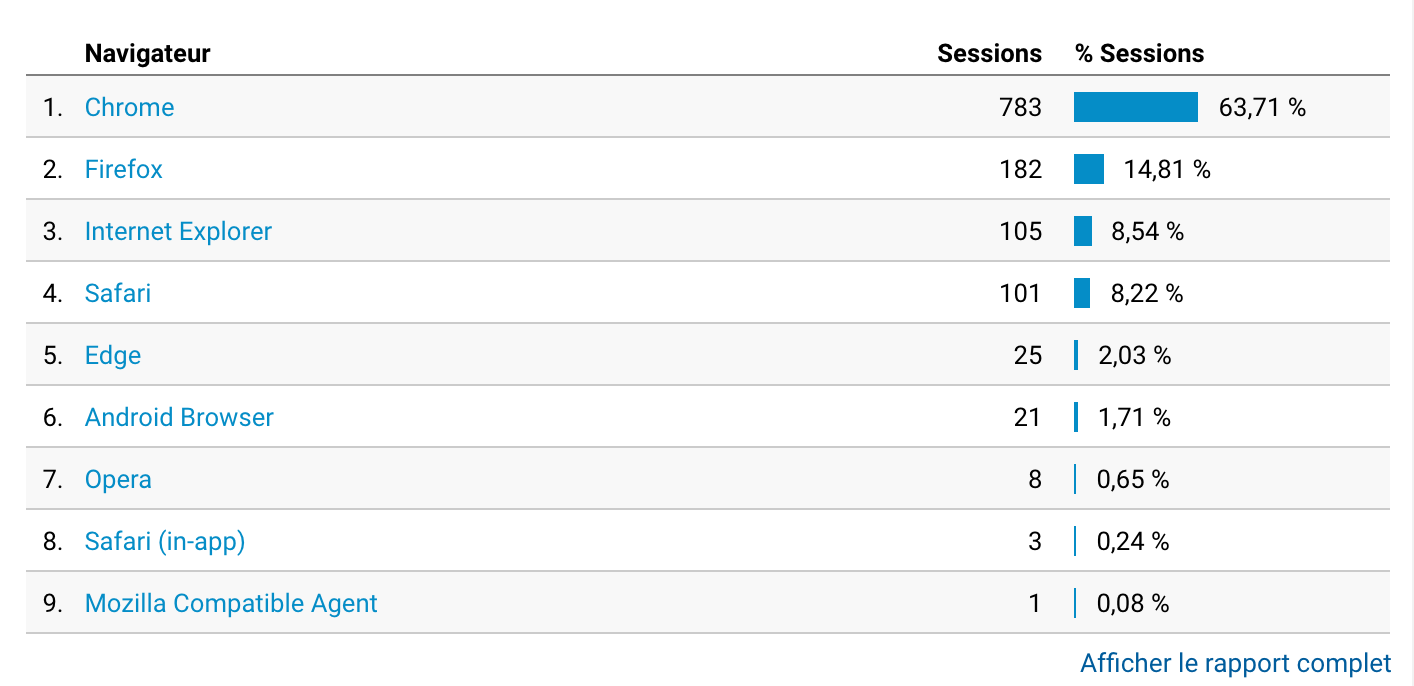
\includegraphics[height=5cm]{figures/FF-browsers.png}
  \caption{Parts de marché des navigateurs Web dans le monde, toutes plates-formes confondues (janvier 2017, source Wikipedia)}
\end{figure}

\bigskip

Une fois que les navigateurs principalement utilisés par la cible sont
identifiés, il faut choisir des outils et méthodes adaptés à ceux-ci. On
peut utilisé des sites comme \href{http://caniuse.com/}{\emph{Can I
use}} qui offre des tableaux de compatibilité pour \emph{HTML5},
\emph{CSS3}, \emph{SVG}, et autres technologies dans les différents
navigateurs. Nous utilisons également
\href{https://www.browserstack.com/}{\emph{BrowserStack}}, un outil de
test multi-navigateurs qui permet aux développeurs de tester leurs sites
web à travers différents navigateurs sur différents systèmes
d'exploitation et appareils mobiles, sans devoir installer de machine
virtuelle. On peut ainsi vérifier le rendu visuel, ainsi que le
comportement de l'application, sur nos navigateurs cibles.

\bigskip

Voici un exemple de problème qu'un développeur peut rencontrer à cause
des différences de comportement entre navigateurs. Après la mise en
place du tunnel de demande de prêt, notre client nous a remonté un
disfonctionnement sur la page de téléchargement de la pièce d'identité.
Sur \emph{Internet Explorer 11} (\emph{IE11}), après le téléchargement,
l'image ne s'affichait pas sur l'interface. Il était alors impossible
pour l'utilisateur de passer à la page suivante. Après de nombreux tests
sur \emph{BrowserStack}, j'ai découvert que \emph{IE11} gardait les
réponses de l'\emph{API} en cache par défaut, c'est à dire les mémoriser
dans l'espace de stockage alloué au navigateur. Quand l'utilisateur
arrivait sur la page, un premier appel à l'\emph{API} était effectué,
afin d'afficher la liste des pièces déjà téléchargées. Cet appel était
mémorisé par le navigateur, et quand l'utilisateur faisait une action
(télécharger une nouvelle pièce d'identité, ou en supprimer une), un
nouvel appel était fait pour récupérer la liste mise à jour. Mais, le
navigateur ignorait cet appel et utilisait à la place le résultat
mémorisé du premier appel. Pour résoudre ce problème, il m'a suffit de
spécifier dans la réponse envoyée par l'\emph{API}, que l'information ne
doit pas être mise en cache. Cela se traduit par l'ajout de la valeur
\texttt{no-cache} au paramètre \texttt{Cache-Control}, dans le
\emph{Header} de la réponse de l'\emph{API}

\bigskip

\paragraph{Génération de contrats}\label{guxe9nuxe9ration-de-contrats}

Au bout d'environ un mois, le développeur présent chez le client a
quitté le projet. Par conséquent, nous avons récupéré la totalité du
développement, tant au niveau du \emph{front} que de l'\emph{API}, ainsi
que la partie administrateur.

\bigskip

Une seconde demande était la mise à jour du contrat généré par
l'application. Après que l'administrateur ait validé la demande de prêt,
un contrat est généré et fourni à l'utilisateur, dans son espace client.
Nous devions mettre à jour les termes du contrat et ajouter des
informations manquantes, de manière dynamique.

\bigskip

Le système de génération de contrats existant était assez rudimentaire
et peu évolutif. Il s'agissait en effet d'une simple concaténation de
chaînes de caractères, et de variables. Il était donc difficile de
modifier le style du contrat, ou même son contenu.

\begin{Shaded}
\begin{Highlighting}[]
\CommentTok{// Ancienne technique pour la génération de contrat}
\KeywordTok{var} \AttributeTok{getContractContent}\NormalTok{() }\OperatorTok{=} \KeywordTok{function} \NormalTok{(loan}\OperatorTok{,} \NormalTok{borrower) }\OperatorTok{\{}
  \KeywordTok{var} \NormalTok{content }\OperatorTok{=} \VerbatimStringTok{`<h2>CE CONTRAT DE PRÊT EST CONCLU}
\VerbatimStringTok{    ENTRE LES SOUSSIGNÉS :</h2><p><b>}
\VerbatimStringTok{    <span style="text-transform: capitalize">`}\OperatorTok{;}
  \NormalTok{content }\OperatorTok{+=} \VariableTok{borrower}\NormalTok{.}\AttributeTok{title} \OperatorTok{+} \VerbatimStringTok{`</span>}
\VerbatimStringTok{   <span style="text-transform: uppercase">`}\OperatorTok{;}
  \NormalTok{conente }\OperatorTok{+=} \VariableTok{borrower}\NormalTok{.}\AttributeTok{last_name}\VerbatimStringTok{`</span>}
\VerbatimStringTok{   <span style="text-transform: capitalize">`}\OperatorTok{;}
  \NormalTok{content }\OperatorTok{+=} \VariableTok{borrower}\NormalTok{.}\AttributeTok{first_name} \VerbatimStringTok{`</span>}
\VerbatimStringTok{    </b> né(e) le <b> `}\OperatorTok{;}
  \NormalTok{content }\OperatorTok{+=} \VariableTok{borrower}\NormalTok{.}\AttributeTok{birthdate} \OperatorTok{+} \VerbatimStringTok{`</b>, à <b> `}\OperatorTok{;}
  \NormalTok{content }\OperatorTok{+=} \VariableTok{borrower}\NormalTok{.}\AttributeTok{birthplace} \OperatorTok{+} \VerbatimStringTok{`</b>, demeurant <b>`}\OperatorTok{;}
  \NormalTok{content }\OperatorTok{+=} \VariableTok{borrower}\NormalTok{.}\AttributeTok{address_line} \OperatorTok{+} \StringTok{' '}
    \OperatorTok{+} \VariableTok{borrower}\NormalTok{.}\AttributeTok{address_postal_code} \OperatorTok{+} \StringTok{' '}
    \OperatorTok{+}  \VariableTok{borrower}\NormalTok{.}\AttributeTok{address_city}\OperatorTok{\}}\NormalTok{\} }\OperatorTok{+} \VerbatimStringTok{`</b>, </p>`}\OperatorTok{;}
\NormalTok{\}}
\end{Highlighting}
\end{Shaded}

\bigskip

Pour résoudre ce problème, nous avons décidé d'utiliser
\href{https://github.com/janl/mustache.js}{\emph{Mustache.js}}, une
librairie de \emph{templating}. Elle permet de mettre en place un
\emph{template HTML} et d'y intégrer facilement nos variables. Il nous
suffit alors de définir un \emph{template} en \emph{HTML}, en y
introduisant le nom de nos variable entre accolades, puis d'appeler la
librairie \emph{Mustache.js} en lui fournissant ce \emph{template} et un
objet, contenant les valeurs de nos variables,
\texttt{Mustache.render(template,\ params)}.

\begin{Shaded}
\begin{Highlighting}[]
\CommentTok{<!-- Extrait du template du contrat -->}
\CommentTok{<!-- .... -->}
\KeywordTok{<h2>}
  \NormalTok{CE CONTRAT DE PRÊT EST CONCLU ENTRE LES SOUSSIGNÉS :}
\KeywordTok{</h2>}
\KeywordTok{<p>}
  \KeywordTok{<b>}
    \KeywordTok{<span}\OtherTok{ style=}\StringTok{"..."}\KeywordTok{>}\NormalTok{\{\{ borrower.title \}\}}\KeywordTok{</span>}
    \KeywordTok{<span}\OtherTok{ style=}\StringTok{"..."}\KeywordTok{>}\NormalTok{\{\{ borrower.last_name\}\}}\KeywordTok{</span>}
    \KeywordTok{<span}\OtherTok{ style=}\StringTok{"..."}\KeywordTok{>}\NormalTok{\{\{ borrower.first_name\}\}}\KeywordTok{</span>}
  \KeywordTok{</b>}
  \NormalTok{né(e) le}
  \KeywordTok{<b>}\NormalTok{\{\{#toDate\}\} \{\{ borrower.birthdate \}\} \{\{/toDate\}\}}\KeywordTok{</b>}\NormalTok{,}
  \NormalTok{à}
  \KeywordTok{<b>}\NormalTok{\{\{ borrower.birthplace \}\}}\KeywordTok{</b>}
  \NormalTok{, demeurant}
  \KeywordTok{<b>}
    \NormalTok{\{\{ borrower.address_line \}\},}
    \NormalTok{\{\{ borrower.address_postal_code \}\}}
    \NormalTok{\{\{ borrower.address_city\}\}}\KeywordTok{</b>}\NormalTok{,}
\KeywordTok{</p>}
\CommentTok{<!-- .... -->}
\end{Highlighting}
\end{Shaded}

\begin{Shaded}
\begin{Highlighting}[]
\CommentTok{// Création d'une variable contenant les paramétres du contrat}
\KeywordTok{var} \NormalTok{getContractParams }\OperatorTok{=} \KeywordTok{function} \NormalTok{(loan}\OperatorTok{,} \NormalTok{borrower) }\OperatorTok{\{}
  \KeywordTok{const} \NormalTok{params }\OperatorTok{=} \OperatorTok{\{}
    \CommentTok{//...}
    \DataTypeTok{borrower}\OperatorTok{:} \NormalTok{borrower}\OperatorTok{,}
    \CommentTok{//...}
  \OperatorTok{\};}
  \ControlFlowTok{return} \NormalTok{params}\OperatorTok{;}
\OperatorTok{\}}
\CommentTok{// Création du contrat avec Mustache.js}
\KeywordTok{var} \NormalTok{getContractContent }\OperatorTok{=} \KeywordTok{function} \NormalTok{(params) }\OperatorTok{\{}
  \KeywordTok{const} \NormalTok{template }\OperatorTok{=} \VariableTok{fs}\NormalTok{.}\AttributeTok{readFileSync}\NormalTok{(}\StringTok{'template.html'}\NormalTok{).}\AttributeTok{toString}\NormalTok{()}\OperatorTok{;}
  \ControlFlowTok{return} \VariableTok{Mustache}\NormalTok{.}\AttributeTok{render}\NormalTok{(template}\OperatorTok{,} \NormalTok{params)}\OperatorTok{;}
\OperatorTok{\}}

\CommentTok{// Récupération des paramétres, création du contrat}
\CommentTok{// et téléchargement sur Amazon S3}
\KeywordTok{var} \NormalTok{createAndUploadContract }\OperatorTok{=} \KeywordTok{function} \NormalTok{(loan}\OperatorTok{,} \NormalTok{borrower) }\OperatorTok{\{}
  \ControlFlowTok{try} \OperatorTok{\{}
    \KeywordTok{var} \NormalTok{contractParams }\OperatorTok{=} \AttributeTok{getContractParams}\NormalTok{(loan}\OperatorTok{,} \NormalTok{borrower)}\OperatorTok{;}
    \KeywordTok{var} \NormalTok{contractContent }\OperatorTok{=} \AttributeTok{getContractContent}\NormalTok{(contractParams)}\OperatorTok{;}
    \AttributeTok{uploadContract}\NormalTok{(contractContent}\OperatorTok{,} \VariableTok{loan}\NormalTok{.}\AttributeTok{id}\NormalTok{)}\OperatorTok{;}
  \OperatorTok{\}} \ControlFlowTok{catch}\NormalTok{(err) }\OperatorTok{\{}
    \VariableTok{logger}\NormalTok{.}\AttributeTok{error}\NormalTok{(}\StringTok{'Error while generating contract'}\NormalTok{)}\OperatorTok{;}
  \OperatorTok{\}}
\OperatorTok{\}}
\end{Highlighting}
\end{Shaded}

\bigskip

\paragraph{Mangopay}\label{mangopay}

L'application \emph{FinFrog} utilise
\href{https://www.mangopay.com/fr/}{\emph{Mangopay}} comme partenaire
pour gérer les transferts d'argent, entre prêteurs et emprunteurs.
\emph{Mangopay} est une solution de paiements dédiée aux
\emph{marketplaces}, plateformes de \emph{crowdfunding} et acteurs de
l'économie collaborative. La société offre à ses clients la possibilité
d'accepter des paiements pour le compte de tiers, de créer et gérer des
\emph{e-wallets}, de répartir les fonds vers de multiples bénéficiaires,
et de collecter automatiquement leurs chiffres d'affaires, le tout de
manière très simple et sécurisé.

\bigskip

J'ai donc dû travailler avec l'\emph{API} de \emph{Mangopay}, notamment
pour gérer l'enregistrement des coordonnées bancaires des utilisateurs.
Pour pouvoir faire cela, un \emph{e-wallet} \emph{Mangopay} est créé
pour chaque utilisateur, à la création de son compte sur \emph{FinFrog}.
Puis, lors de la récupération de l'IBAN et des informations de la carte
bancaire de l'utilisateur, nous associons à ce \emph{e-wallet} la carte
et le compte bancaire. Les informations de la carte bancaire sont
envoyées directement à \emph{Mangopay} car, pour des raisons de
sécurité, nous ne pouvons pas faire transiter ces dernières vers
l'\emph{API}. Une fois la carte enregistrée, nous créons une
pré-authorisation associée. Une pré-autorisation est une action qui
permet de vérifier si l'utilisateur à une certaine capacité financière
sur son compte bancaire. Cela nous permet donc de vérifier s'il sera en
mesure de rembourser son prêt ou non.

\bigskip

Il est également nécessaire de fournir à \emph{Mangopay} de nombreuses
informations sur l'utilisateur, dans le cadre du \emph{KYC}. Le
processus \emph{Know Your Customer} est utilisé dans le but d'assurer
que les clients sont conformes aux lois anti-corruption. Cela a
également pour but de prévenir l'usurpation d'identité, la fraude
financière, le blanchiment d'argent et le financement du terrorisme.
C'est un processus donc très important dans le cadre d'entreprises comme
\emph{FinFrog}, qui gèrent des flux quotidiens d'argent. Pour répondre
au \emph{KYC}, nous fournissons, en plus des informations de base (date
et lieu de naissance, adresse, etc.), les pièces d'identité récupérées
lors de la demande de prêt.

\bigskip

\paragraph{Fin du stage}\label{fin-du-stage}

Quelques semaines avant la fin de mon stage chez \emph{Dernier Cri},
\emph{FinFrog} a accueilli un nouveau développeur sur le projet, engagé
par le client. Pour lui permettre de découvrir et appréhender
correctement le projet, nous lui avons présenté notre travail sur le
projet, dans nos locaux. Au cours de cette journée, nous lui avons
présenté tout les aspects de \emph{FinFrog}, de l'infrastructure, aux
flux entre le site et l'\emph{API}, en passant par notre gestion de
projets.

\bigskip

Pendant la fin du stage nous avons mis en place avec lui un plan
d'amélioration du code de l'application. En effet, le projet ayant était
développer assez rapidement par le premier développeur de
\emph{FrinFrog}, certain choix de conception ne sont aujourd'hui plus
pertinant. Nous avons également besoin de nouveaux outils: générer une
documentation à partir des commentaires de l'application, mettre en
place des migrations pour la bases de données etc.

\bigskip

C'est également à ce moment que le mode de facturation du projet est
passé de forfait à régie. Auparavant, en mode forfait, nous devions
estimé chaque tâche, et les dépassements n'étaient pas facturés. En mode
régie, le tout temps de développement est facturé. D'une part cela
signifie que le client est satisfait de notre travail et nous fait
confiance, d'autre part cela nous permet d'avoir une plus grande liberté
de mouvement: nous ne devons plus attendre une estimations et une
validations avant de se lancer dans un développement.

\bigskip

\subsubsection{Conclusion}\label{conclusion-1}

\emph{FinFrog} a été un projet très enrichissant, car abordant de
nombreuses problématiques pouvant être rencontrées dans le développement
web, et utilisant de nombreux outils.

\bigskip

J'ai eu l'opportunité de participer activement aux réflexions concernant
la conception du site. En effet, notre client était ouvert au
suggestions et remarques, et tenait à se que nous comprenions les
tenants et aboutissants de chaque décision et des nouveaux
développements. C'est pour cela que nous avions de nombreuses réunions
téléphoniques, et débat écrits. J'ai ainsi pu appréhender les
problématiques des \emph{Fintech}, ses entreprises qui utilisent la
technologie pour lancer des services bancaires et financiers
innovants.\\
Cela m'a également permis de travailler sur mon relationnel client,
grâce au contact presque journalier avec notre client pour récolter ses
besoins, puis ses retours par rapport aux fonctionnalités développées.

\bigskip

Grâce à ce projet j'ai également pu découvrir de nombreux outils, plus
ou moins importants, comme le service \emph{Mangopay}, des outils de
\emph{monitoring} comme \emph{Google Analytics} ou \emph{Hotjar}, ou
encore de nombreuse librairie comme \emph{Mustache.js}, \emph{Redux
Form} ou encore \emph{React Router}.

\bigskip

\subsection{Autre projet : Générateur d'images pour Dernier
Cri.}\label{autre-projet-guxe9nuxe9rateur-dimages-pour-dernier-cri.}

\bigskip

Comme dit précédemment, \emph{Dernier Cri} possède un blog tenu par ses
développeurs. L'équipe essaye de tenir un rythme de publication d'un
article par semaine. Pour faire la promotion de cette activité,
\emph{Dernier Cri} partage les publications sur les réseaux sociaux.

\bigskip

Pour permettre une meilleure communication, il est venue l'idée de créer
des images personnalisées pour chaque article, qui seraient utilisées
sur les réseaux sociaux. Evidemment, la création de ces images serait
automatisée. J'ai décidé de relever ce défi et de créer ce générateur
d'images.

\bigskip

J'ai tout d'abord choisi, sur les conseils de mon tuteur d'entreprise,
d'utiliser
\href{https://www.imagemagick.org/script/index.php}{\emph{ImageMagick}}
pour générer mes images. \emph{ImageMagick} est un logiciel libre,
comprenant une bibliothèque, ainsi qu'un ensemble d'utilitaires en ligne
de commande, permettant de créer, convertir, modifier et afficher des
images dans un très grand nombre de formats. Il offre de nombreuses
possibilités pour manipuler les images: il est possible de les découper,
de modifier leurs couleurs, de leur faire faire des rotations, d'y
inclure du texte, etc.\\
J'ai donc commencé par prendre en main \emph{ImageMagick} en ligne de
commande, pour doucement créer l'image voulue grâce à un script
\emph{bash}.

\bigskip

Dans ce script, je construisais mon image finale par étape :

\begin{itemize}
\tightlist
\item
  Création de l'image de fond : tout d'abord il fallait redimensionner
  l'image choisie comme image de fond, puis y appliquer un filtre bleu
  pour obtenir l'effet souhaité.
\end{itemize}

\begin{verbatim}
# Creation du filtre bleu
convert -size 600x315 xc:rgb\(0,44,92\) blue.png

# Redimensionnement et filtre
convert -resize ${width}x${height} background.jpg background.png
convert background.png -colorspace Gray background.png
composite -blend 90% -gravity South blue.png background.png
\end{verbatim}

\begin{itemize}
\item
  La création de l'image de l'auteur: je récupère l'image de l'auteur de
  l'article, puis utilise un masque pour la rendre ronde.

\begin{verbatim}
# Création de l'image de l'auteur
convert JS.jpg  -resize $userWidth \
\( +clone -threshold -1 -negate -fill white -draw \
"circle `expr $userWidth / 2`,
`expr $userWidth / 2`, `expr $userWidth / 2`,0" \) \
-alpha off -compose copy_opacity -composite xavier.png
\end{verbatim}
\item
  Création des différents textes : je créé ensuite le titre de l'image,
  ainsi que la signature comprenant le nom de l'auteur ainsi que sa
  fonction chez \emph{Dernier Cri}.
\item
  Il suffit enfin de superposer les différents éléments pour créer
  l'image souhaitée.
\end{itemize}

\begin{figure}[h]
  \centering
  
\includegraphics[height=6cm]{figures/blog.png}
  \caption{Image générée pour un article de blog}
\end{figure}

\bigskip

Une fois le processus maitrisé en ligne de commande, j'ai pu commencer à
l'intégré au site web de \emph{Dernier Cri}. Ce dernier étant développé
en \emph{Ruby on Rails}, j'ai tout d'abord dû me familiariser avec cette
pile technologique, à travers différents tutoriels, avant de pouvoir
coder ce générateur.

\bigskip

Pour intégrer le processus de génération d'images au site web, j'ai
utilisé \href{https://github.com/rmagick/rmagick}{\emph{RMagick}}, une
bibliothèque servant d'interface entre le langage \emph{Ruby} et la
bibliothèque \emph{ImageMagick}. J'ai donc pû traduire mon processus de
création d'images en \emph{Ruby}, et l'intégrer au site sans
difficultés.\\
Voici un exemple de traduction, avec la superposition du logo de
\emph{Dernier Cri} sur l'image de fond :

\begin{Shaded}
\begin{Highlighting}[]
\CommentTok{# Script Image Magick}
\ExtensionTok{composite} \NormalTok{\textbackslash{}}
  \DataTypeTok{\textbackslash{}(} \NormalTok{logo.png -resize x}\VariableTok{$logoHeight} \DataTypeTok{\textbackslash{})} \NormalTok{\textbackslash{}}
  \NormalTok{-gravity NorthEast -geometry +10+10 background.png background.png}
\end{Highlighting}
\end{Shaded}

\begin{Shaded}
\begin{Highlighting}[]
\CommentTok{# Traduction en Ruby}
\KeywordTok{def} \NormalTok{add_logo(background)}
  \NormalTok{logo = }\DataTypeTok{Magick}\NormalTok{::}\DataTypeTok{Image}\NormalTok{.from_blob(}
    \NormalTok{open(}\DataTypeTok{Settings}\NormalTok{.blog_post_cover.logo_url).read}
  \NormalTok{).first}

  \NormalTok{background.composite!(}
    \NormalTok{logo,}
    \DataTypeTok{Magick}\NormalTok{::}\DataTypeTok{NorthEastGravity}\NormalTok{,}
    \DecValTok{10}\NormalTok{,}
    \DecValTok{10}\NormalTok{,}
    \DataTypeTok{Magick}\NormalTok{::}\DataTypeTok{AtopCompositeOp}
  \NormalTok{)}
\KeywordTok{end}
\end{Highlighting}
\end{Shaded}

\bigskip

Les articles du blogs sont stockés et gérés sur \emph{Contenful}, un
système de gestion de contenu. C'est donc en interfaçant mon programme
avec \emph{Contenful} que je peux récupérer les informations nécessaires
à la génération d'images: le titre de l'article, son auteur, sa photo,
etc.

\bigskip

La génération de l'image terminée, j'ai dû mettre en place un service
pour garder en mémoire cette image, et ne pas la régénérer à chaque
partage. Pour cela, j'ai utilisé \emph{CloudFront} de \emph{AWS}
(\emph{Amazon Web Service}) qui permet de garder en cache l'image après
le premier appel. En effet, je fourni pour le partage comme adresse de
l'image le nom de domaine de mon \emph{CloudFront}, avec le nom de mon
image (par exemple \texttt{http://XXXXX.cloudfront.net/monoide}).\\
Voici ce qu'il se passe lorsque l'on contacte cette \emph{URL}:

\begin{itemize}
\item
  Si mon image n'a jamais été générée, et donc que \emph{CloudFront} ne
  l'a pas dans son cache, le service va faire un appel au site
  \emph{Dernier Cri}, sur l'adresse du générateur, pour récupérer cette
  image, la retourner et la mémoriser.
\item
  Lors des prochains appels, \emph{CloudFront} pourra retourner
  directement l'image, et donc éviter de redemander sa génération.
\end{itemize}

\bigskip

Finalement, pour que l'image soit utilisée sur les réseaux sociaux, il
m'a suffit d'ajouter l'adresse de mon image dans \emph{CloudFront},
directement dans les balises des pages associées aux articles de blog.

\begin{figure}[h]
  \centering
  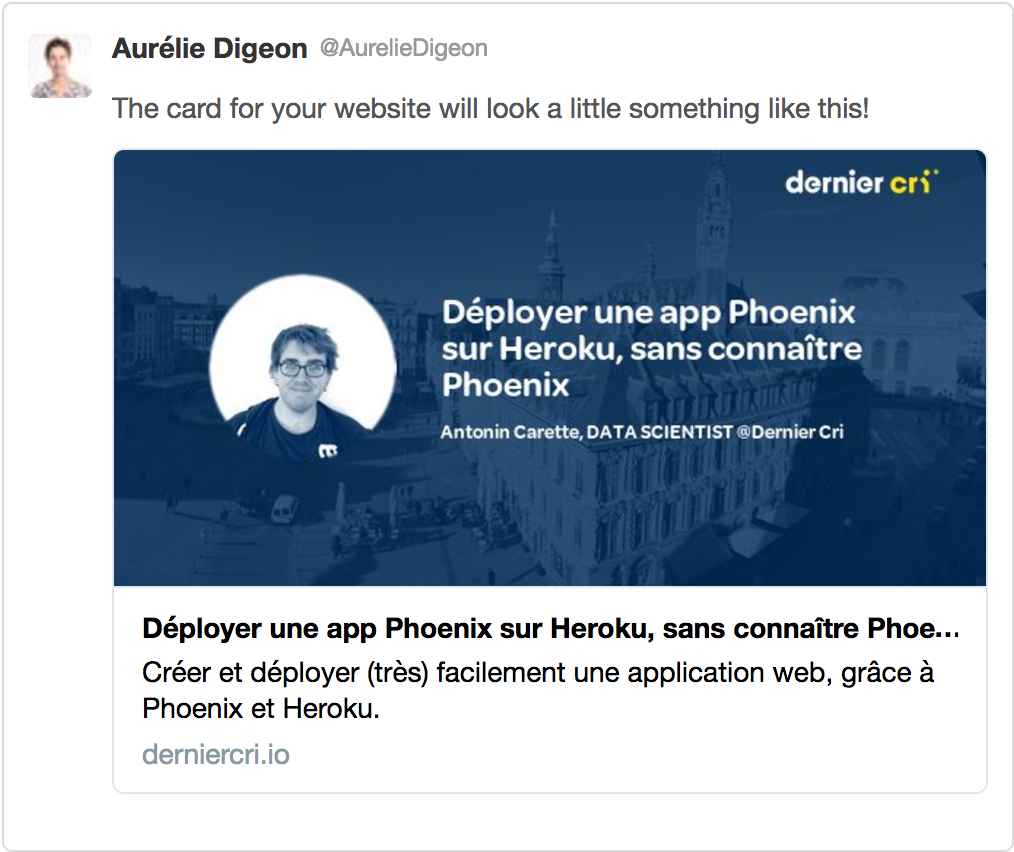
\includegraphics[height=6cm]{figures/partage-blog.png}
  \caption{Exemple de partage d'article sur Twitter}
\end{figure}

\newpage

\section{La communauté Lilloise}\label{la-communautuxe9-lilloise}

Durant mon stage à Lille j'ai pu me rendre compte que la ville possédait
une communauté web très active.

\bigskip

La ville a notamment reçue le label \emph{French Tech} fin 2014, pour
récompenser son dynamiste dans le numérique et l'innovation. Ce label,
en plus de récompenser les efforts de la ville, constitue le point
d'entrée vers des dispositifs nationaux comme des programmes pour
attirer les entrepreneurs étrangers qui veulent créer leur
\emph{startup} en France.

\bigskip

La région profite de la présence de grands groupes nationaux comme
Orange, Capgemini, IBM France, CGI, CISCO\ldots{}

\bigskip

De plus Lille a mis en place un ensemble de structures favorisant
l'accompagnement et la croissance des startups vers un marché mondial.
La plus notable est évidemment Euratechnologie, le Pôle d'excellence
économique dédié aux Technologies de l'Information et de la
Communication (TIC) de la métropole lilloise. EuraTechnologies a été
classé dans le top 10 des accélérateurs de \emph{startup} d'Europe par
Fundacity, et le 1er en France. Euratechnologie posséde des espaces
dédiés à la recherche, la formation et l'entrepreneuriat, un incubateur
et un accélérateur.

\bigskip

La région lilloise posséde d'autre espaces dédié à l'innovation, les
\emph{startups} et l'entrepreneuriat : La Plaine Images à Tourcoing et
Roubaix, Eurasanté à Lille, La Haute Borne à Villeneuve d'Ascq, La Serre
Numérique à Valenciennes, Le Pôle Numérique Culturel Louvre Lens\ldots{}

\bigskip

La région a connu l'émergence de nombreuse entreprises, prometteuses ou
déjà fructueuses : Big Ben, Ankama, OVH, Addictiz, Stereograph, Clic \&
Walk, Giroptic, Mazeberry, Vekia, Sparkow, Mdoloris, A-volute, Critizr,
Intent Technologies\ldots{}

\bigskip

Avoir eu la chance de faire mon stage dans cette région m'a permis de
profiter de cette écosysteme riche et actif. J'ai pu participer à des
conférences, des salons et des réunions qui m'ont beaucoup apporté, tant
au niveau technique que social. Cela m'a permit de préciser mon projet
professionnel, en m'immergeant dans la vie entreprenariale d'une ville.

\bigskip

\subsection{Take Off Conference}\label{take-off-conference}

\bigskip

\emph{Dernier Cri} m'a donné l'occasion durant mon stage d'assister à la
\href{http://takeoffconf.com/2016}{\emph{Take Off Conference}} les 20 et
21 octobre 2016. Cet évènement a lieu depuis plusieurs années à
EuraTechnologies.

\bigskip

Historiquement, ce sont les fondateurs de \emph{Dernier Cri} qui ont
créé la \emph{Take Off Conference}, avec Florian Le Goff. Aujourd'hui ce
sont d'autres acteurs de la communauté web de Lille qui ont pris le
relais pour proposer une nouvelle édition.

\bigskip

La \emph{Take Off Conference} est un cycle de conférences anglophones.
L'événement dure 2 jours, et accueille des conférenciers du monde
entier. Bien qu'elle reste avant tout une conférence pour les
développeurs Web, elle reste accessible pour les développeurs en
général.

\bigskip

\emph{Dernier Cri} m'a permis de participer à cette conférence avec l'un
de mes collègues. Ce fut une véritable chance pour moi de rencontrer et
échanger avec des conférenciers du monde entier. Les conférences étaient
très intéréssantes et inspirantes, sur des sujets très variés allant de
la compréhension des enjeux de mise en place de nouveau outils, à des
sujets plus sociaux comme l'acceuil des developpeurs anglais après le
Brexit.

\bigskip

Des évènements ont également été organisé le soir pour permettre aux
participants et aux conférenciers d'échanger dans un cadre plus détendu.

\bigskip

Ce fut une excellente occasion de découvrir de nouvelles technologies,
de m'ouvrir à des problématiques que je ne connaissais pas ainsi que de
rencontrer des développeurs qualifiés et passionnés. Lors de ses
échanges, j'ai pu me rendre compte de la portée internationale de la
programmation : des personnes des quatres coins du monde se retrouvaient
sur les mêmes problématiques.

\bigskip

\subsection{Meetup}\label{meetup}

\bigskip

La communauté web de Lille est très active pour organisé des évenements.
De très nombreux Meetup sont organisés sur différents domaines du web,
acceuillant autant des experts que des débutants ou simplement des
curieux.

\bigskip

Très actif dans cette communauté, \emph{Dernier Cri} acceuille au sein
de ses locaux certaines de ses rencontres. J'ai notamment eu l'occasion
d'assister à des \emph{Meetups} de \emph{Lille FP} (\emph{Fonctionnal
programming}, c'est à dire programmation fonctionnelle) et de
\emph{Lille Elixir}.

\bigskip

Certains membres de l'équipe sont également investis dans ces
rencontres, en tant qu'organisateur ou bien orateur. Les dirigeants de
\emph{Dernier Cri} les encouragent également beaucoup à prendre part à
la vie de la communauté web. J'ai ainsi pu facilement être au courant
des différents évenements Lillois et y participer avec mes collégues, ce
qui m'a permis d'être bien intégré.

\bigskip

\subsection{Maker Faire}\label{maker-faire}

\bigskip

La Maker Faire est un autre événement majeur organisé à Lille durant mon
stage. Ce concept totalement unique regroupe stands de démonstration,
ateliers de découverte, spectacles et conférences autour des thèmes de
la créativité, de la fabrication, des cultures Do It Yourself et Makers.

\bigskip

Cet événement, présenté par Leroy Merlin en partenariat avec la Ville de
Lille et lille3000 (programme culturel de la ville de Lille), réunit des
passionnés de technologies, des artisans, des industriels, des amateurs,
des ingénieurs, des clubs de science, des artistes, des étudiants et des
Start'Up. Ils forment la communauté des Makers et viennent pour montrer
leurs créations, partager leurs connaissances\ldots{}

\bigskip

\emph{Dernier Cri} a été invité à assister à la Maker Faire, notamment
car nous développons l'application web de TechShop, l'atelier
collaboratif de Leroy Merlin. Dans ce contexte j'ai pu découvrir la
communauté \emph{Maker} de Lille. J'ai pu notamment décrouvrir les
\emph{repair coffee}, lieux où l'on peut amener ses appareils
électroniques cassés et recevoir de l'aide pour leur réparation. Il y
avait également des robots, des imprimantes 3D, des casques de réalité
augmentée \ldots{} C'était un endroit plein d'inspiration et d'envie
d'entreprendre.

\newpage

\section{Conclusion}\label{conclusion-2}

Ce stage chez \emph{Dernier Cri} et ma participation aux projets
\emph{Photolix} et \emph{FinFrog} ont été très enrichissante. J'ai pu
mettre en application

\bigskip

Ce stage a été très enrichissant pour moi. Il m'a permit de participer
au développement d'application web, , à travers les projets
\emph{Photolix} et \emph{FrinFrog}, sous la houlette d'une équipe
expérimentécomplet qui à su me transmettre des compétences techniques et
méthodologiques.\\
J'ai notamment pu prendre en main de nombreuses bibliothéques, comme
\emph{React}, \emph{Redux}, des langages comme \emph{Ruby on Rails} ou
encore travailler avec des partenaires comme \emph{Mangopay}.

\bigskip

J'ai aussi pu découvrir la réalité des entreprises et appliquer les
notions acquises à l'université, apprendre ou de me perfectionner avec
certaines technologies ou méthodes et de développer l'aptitude au
travail en équipe.

\bigskip

Enfin, vous pouvez re-situez votre stage dans votre parcours de
formation et dans votre projet professionnel. Vos objectifs ont-ils
évolué ? Par exemple, en quoi ce stage confirme (ou infirme) votre choix
de filière ?

-\textgreater{} Compétences apprises : Node React Redux ES6 Relation
client Git Github pm2 npm

-\textgreater{} Important : relation client et autonomie, apprentissage
rapide, equipe disponible et polivalente (qui peut t'aider sur tout)

-\textgreater{} environnement cool : Ambiance, tech off conf , meetup,
plus belle vue de Lille

\newpage

\section{Glossaire}\label{glossaire}

\textbf{Account manager:} c'est un intermédiaire entre l'entreprise et
le client. Il cherche de nouveaux clients, prend note de leurs besoins
et identifie ensuite le produit ou le service qui y répond le mieux. Il
essaie également de fidéliser les clients actuels en leur fournissant un
service après-vente optimal.

\bigskip

\textbf{API}(\emph{Application Programming Interface})\textbf{:} c'est
une interface de programmation applicative, c'est à dire un ensemble
normalisé de classes, de méthodes ou de fonctions qui qui permet à un un
logiciel de fournir des services à d'autres logiciels.

\bigskip

\textbf{Back} Partie de l'application non accessible aux utilisateurs
finaux, elle communique avec le \emph{front} pour lui fournir des
services.

\bigskip

\textbf{CEO} (\emph{chief executive officer})\textbf{:} directeur
général d'une entreprise.

\bigskip

\textbf{Chatops:} outil d'administration d'infrastructure par la
discussion.

\bigskip

\textbf{Code review} (Revu de code) \textbf{:} examen systématique du
code source, pour vérifier le respect d'un ensemble de règles de
programmation, trouver des bugs, corriger des erreurs de conception,
améliorer la qualité, la maintenabilité et la sécurité.

\bigskip

\textbf{Crowdfunding:} (financement participatif) expression décrivant
tous les outils et méthodes de transactions financières qui font appel à
un grand nombre de personnes afin de financer un projet.

\bigskip

\textbf{CTO} (\emph{Chief Technology Officer})\textbf{:} directeur
technique, chargé de s'occuper de la direction des questions
scientifiques et techniques.

\bigskip

\textbf{Data scientist :} (scientifique de données) expert de la gestion
et de l'analyse pointue de données massives (``big data''). Il détermine
des indicateurs permettant la mise en place d'une stratégie à partir de
sources de données multiples et dispersées.

\bigskip

\textbf{Devops:} employé doté des compétences nécessaires pour
travailler à la fois en tant que développeur et ingénieur système.

\bigskip

\textbf{DOM} (\emph{Document Object Model})\textbf{:} interface de
programmation qui fournit une réprésentation du contenue de la page web
pour permettre à des scripts d'examiner et de modifier son contenu.

\bigskip

\textbf{ECMAScript:} ensemble de normes concernant les langages de
programmation de type script et standardisées par Ecma International.

\bigskip

\textbf{E-wallet:} dispositif électronique qui permet à un individu de
faire des transactions électroniques.

\bigskip

\textbf{Fintech:} contraction de `Finance' et `Technologie', c'est un
domaine d'activité dans lequel les entreprises utilisent les services
informatique pour fournir des services financiers.

\bigskip

\textbf{Framework:} ensemble d'outils et de composants logiciels à la
base d'un logiciel ou d'une application.

\bigskip

\textbf{Front:} partie de l'application accessible aux utilisateurs
finaux, qui permet d'interagir avec les reste de l'application (le
\emph{back}).

\bigskip

\textbf{Git:} logiciel de gestion de versions décentralisé.

\bigskip

\textbf{Immutable:} Se dit des types de variables qui ne peuvent pas
changer de valeur pendant l'exécution du programme.

\bigskip

\textbf{Marketplace:} plateforme dont l'objectif est de mettre en
relation des vendeurs et des acheteurs, particuliers ou professionnels.

\bigskip

\textbf{Mise en production:} déployer des modifications sur la version
du projet accéssible aux utilisateurs finaux.

\bigskip

\textbf{Monitoring:} supervision de l'application par la mesure de
divers indicateurs (nombre d'erreur, temps de réponse etc.).

\bigskip

\textbf{Open source:} programme informatique dont le code source est
distribué sous une licence permettant à quiconque de lire, modifier ou
redistribuer ce logiciel.

\bigskip

\textbf{Recette:} phase de test des nouvelles fonctionnalités, visant à
s'assurer que le produit est conforme aux spécifications.

\bigskip

\textbf{Routage:} sélection des chemins dans un réseau pour acheminer
les données d'un expéditeur jusqu'à un ou plusieurs destinataires.

\bigskip

\textbf{Startup:} jeune entreprise innovante à fort potentiel de
croissance, ou entreprise en construction.

\bigskip

\textbf{Template:} est un élement qui fait office de gabarit (modèle) où
seuls certains éléments sont modifiables (le contenu texte, les images,
les couleurs etc\ldots{}).
